% Tratto da grfguide.[ps|pdf]:
%
%\graphicspath{<dir-list>}
%    This optional declaration may be used to specify a list of directories in which to search
%    for graphics files. The format is the same as for the LATEX 2e primitive \input@path.
%    A list of directories, each in a {} group (even if there is only one in the list). For example:
%    \graphicspath{{eps/}{tiff/}}
%    would cause the system to look in the subdirectories eps and tiff of the current directory.
%
%\graphicspath{{FIGS/}}
%
% E` preferibile fare come segue, perche' in questo modo ad es. anche i .tex
% possono essere messi in altre directory e inclusi senza indicarne il percorso.
\makeatletter
\let\input@path=\@undefined
\def\input@path{{FIGS/}}
\makeatother

\ifx\pdfoutput\undefined % We are not running pdftex
\documentclass[12pt,a4paper]{report}

\usepackage[dvips]{graphicx,color}
% \usepackage{psfig}
% \usepackage{epsfig}
\DeclareGraphicsExtensions{.ps,.eps,.pstex}
% Use the following line if you want to obtain a .pdf through dvipdfm
% (.tex -(latex)-> .dvi -(dvipdfm)-> .pdf)
\RequirePackage[dvipdfm,hyperindex]{hyperref}
% % \RequirePackage[dvipdfm,colorlinks,hyperindex]{hyperref}
% Use the following two lines if you want to obtain a .pdf with hyperlinks
% also through ps2pdf (.tex -(latex)-> .dvi -(dvips)-> .ps -(ps2pdf)-> .pdf)
% (this can be useful if you want to use Inkscape and PSFrag to put
%  equations in the figure)
% \RequirePackage[hyperindex]{hyperref}
% \usepackage{psfrag}
% % \RequirePackage[hypertex]{hyperref}
\else % We are running pdftex
\documentclass[pdftex,12pt,a4paper]{report}
\usepackage[pdftex]{graphicx,color}
\DeclareGraphicsExtensions{.pdf,.png,.jpg,.mps}
\RequirePackage[hyperindex]{hyperref}
% % \RequirePackage[colorlinks,hyperindex]{hyperref}
% % \usepackage{thumbpdf}
\hypersetup{
pdftitle={Sperimentazione di reti wireless mobili mediante virtualizzazione container-based ed emulazione in tempo reale del canale},
pdfsubject={Tesi Laurea Triennale},
pdfauthor={Fabio Di Sabatino},
pdfkeywords={Modello, tesi, LaTeX, PDF, Howto, pdflatex, dvipdfm},
% pdfpagemode=FullScreen
}
\fi

\usepackage{times}
%\usepackage{mathptmx}
\usepackage[scaled=.90]{helvet}
\usepackage{courier}

\textwidth	140 mm
\textheight	210 mm
\headheight	 10 mm
\headsep	  8 mm
\hoffset	 14.6 mm
\oddsidemargin	  0 mm
\voffset	  9.6 mm
\topmargin	  0 mm
\renewcommand{\baselinestretch}{1.14}
% \renewcommand{\baselinestretch}{1}
% \baselineskip = 20 pt

\date{~}
\newlength{\defaultparindent}
\setlength{\defaultparindent}{\parindent}

\usepackage{enumerate}
\usepackage{float}

\usepackage[italian]{babel}
\usepackage[utf8x]{inputenc}
%\usepackage[latin1]{inputenc}
%\usepackage[applemac]{inputenc}

\frenchspacing

\usepackage{amssymb,amstext,amsmath}
%\usepackage{bigint}
%\usepackage{esint}
\usepackage{multirow}
\usepackage{listings}
\usepackage{color}

\newcommand{\ty}{\tilde{y}}
\newcommand{\tM}{\widetilde{M}}
\newcommand{\tSIR}{\text{SIR}}
\newcommand{\tout}{\text{out}}
\newcommand{\thit}{\text{hit}}
\newcommand{\thop}{\text{hop}}
\newcommand{\setawn}{\left( \sigma_{w_n} , \eta_{w_n} \right)}
\newcommand{\var}{\text{var}}
%\def\myvector#1{\underline{#1}}
%\def\myversor#1{\hat{\underline{#1}}}
\newcommand{\myvector}[1]{\underline{#1}}
\newcommand{\myversor}[1]{\hat{\underline{#1}}}
%\newcommand{\myvector}[1]{\text{\boldmath $#1$}}
%\newcommand{\myversor}[1]{\hat{\text{\boldmath $#1$}}}
%\newcommand{\mymatrix}[1]{\text{\boldmath $#1$}}
\newcommand{\mymatrix}[1]{\pmb{#1}}
\newcommand{\erf}{\text{erf}}
\newcommand{\erfc}{\text{erfc}}
\newcommand{\erfinv}{\text{erfinv}}
\newcommand{\inverf}{\text{inverf}}
\newcommand{\rect}{\text{rect}}
\newcommand{\rep}{\text{rep}}
\newcommand{\sinc}{\text{sinc}}
\newcommand{\sgn}{\text{sgn}}
\newcommand{\conv}{\otimes}
\newcommand{\T}{\mathbb{T}}
\newcommand{\R}{\mathbb{R}}
\newcommand{\Z}{\mathbb{Z}}
\newcommand{\C}{\mathbb{C}}
\newcommand{\F}{\mathcal{F}}

\RequirePackage{fancyhdr}
\pagestyle{fancy}
\fancyhf{}
%\renewcommand{\chaptermark}[1]{\markboth{\scshape \chaptername\ \thechapter\ -- #1}{}}
\renewcommand{\chaptermark}[1]{\markboth{\chaptername\ \thechapter\ -- #1}{}}
\fancyhead[L]{\leftmark}
\fancyhead[R]{\thepage}

% Per far numerare anche le subsubsection:
\setcounter{secnumdepth}{3} % il default è 2 e quindi comprende fino alle subsection
% Per far inserire anche le subsubsection nella Table Of Contents:
\setcounter{tocdepth}{3}    % il default è 2 e quindi comprende fino alle subsection

\usepackage{verbatim}

%%MY STYLES
%%%%%%%%%%%
%%  XML  %%
%%%%%%%%%%%
\definecolor{gray}{rgb}{0.4,0.4,0.4}
\definecolor{darkblue}{rgb}{0.0,0.0,0.6}
\definecolor{cyan}{rgb}{0.0,0.6,0.6}
\DeclareFixedFont{\ttb}{T1}{txtt}{bx}{n}{12} % for bold
\DeclareFixedFont{\ttm}{T1}{txtt}{m}{n}{12}  % for normal
\definecolor{deepblue}{rgb}{0,0,0.5}
\definecolor{deepred}{rgb}{0.6,0,0}
\definecolor{deepyellow}{rgb}{0.6,0.6,0}
\definecolor{deepgreen}{rgb}{0,0.5,0}

\lstset{
  basicstyle=\ttfamily,
  columns=fullflexible,
  showstringspaces=false,
  commentstyle=\color{gray}\upshape,
  breaklines=true,
}

\lstdefinelanguage{XML}
{
  morestring=[b]",
  morestring=[s]{>}{<},
  morecomment=[s]{<?}{?>},
  stringstyle=\color{black},
  identifierstyle=\color{darkblue},
  keywordstyle=\color{cyan},
  morekeywords={xmlns,version,type}% list your attributes here
}
\lstdefinelanguage{JavaScript}{
  keywords={typeof, new, true, false, catch, function, return, null, catch, switch, var, if, in, while, do, else, case, break},
  keywordstyle=\color{blue}\bfseries,
  ndkeywords={class, export, boolean, throw, implements, import, this},
  ndkeywordstyle=\color{darkblue}\bfseries,
  identifierstyle=\color{black},
  sensitive=false,
  comment=[l]{//},
  morecomment=[s]{/*}{*/},
  commentstyle=\color{red}\ttfamily,
  stringstyle=\color{red}\ttfamily,
  morestring=[b]',
  morestring=[b]"
}
%%%%%%%%%%%
%%  PHP  %%
%%%%%%%%%%%
\lstdefinelanguage{PHP}
{
  morestring=[b]",
  morestring=[s]{"}{"},
  stringstyle     =\color{deepgreen},
  identifierstyle =\color{black},
  otherkeywords   = {fopen, fclose, bcadd, fwrite, bccomp, bcsub, true, false, ksort, isset, fgets, round, substr, preg_match, feof, trim, explode},   
  keywordstyle    =\color{darkblue},
  commentstyle    = \color{gray},
  emph            =[1]{php, <?php, ?>},
  emphstyle       =[1]\color{black},
  emph            =[2]{if,and,or,else,while,for, foreach, as},
  emphstyle       =[2]\color{deepred}
}

%%%%%%%%%%%%
%%  BASH  %%
%%%%%%%%%%%%
\lstdefinelanguage{BASH}
{
  stringstyle=\color{black},
  identifierstyle=\color{darkblue},
  commentstyle=\color{red},
  keywordstyle=\color{blue},
  morekeywords={xmlns,version,type}% list your attributes here
}

%%%%%%%%%%%%
%% PYTHON %%
%%%%%%%%%%%%
\lstdefinelanguage{PYTHON}
{
  morestring=[s]{"}{"},
  stringstyle=\color{deepgreen},
  identifierstyle =\color{black},
  basicstyle=\ttm,
  otherkeywords={self, import, def, class, except, open, while, str, handle.write, handle.close},             % Add keywords here
  keywordstyle=\ttb\color{deepblue},
  emph={MyClass,__init__},          % Custom highlighting
  emphstyle=\ttb\color{deepred},    % Custom highlighting style
  frame=tb,                         % Any extra options here
  showstringspaces=false,           % 
}

\begin{document}

\renewcommand{\figurename}{\small Figura}
\renewcommand{\tablename}{\small Tabella}

% BEGIN Frontespizio
\begin{titlepage}

\begin{center}
\normalsize

\begin{center}
\begin{tabular}[t]{@{} l @{} c @{} r @{}}
\parbox[c]{0.15\textwidth}{\raggedright 
\includegraphics[width=0.60in]{logo_univ}}
&
\parbox[c]{0.7\textwidth}
{
\centering \bfseries
UNIVERSITÀ DEGLI STUDI DELL'AQUILA \\[-5pt]
\rule{0.65\textwidth}{1pt} \\
{\scshape DIPARTIMENTO DI \\ INGEGNERIA E SCIENZE DELL'INFORMAZIONE E MATEMATICA }
}
&
\parbox[c]{0.15\textwidth}{\raggedleft 
\includegraphics[width=0.70in]{logo_ing}}
\end{tabular}
\end{center}

\bigskip \bigskip



\bigskip \bigskip

{\small CORSO DI LAUREA IN} \\
INGEGNERIA DELL'INFORMAZIONE

\vfil \vfil \vfil

{\bfseries \large
Un'applicazione mobile geolocalizzata cross-platform per contesti di disaster-management\\
}

\vfil \vfil \vfil

\makebox[\textwidth][c]{

\begin{minipage}[t]{0.4\textwidth}
\centering
{\bfseries Relatrice:} \\
{\itshape Prof.ssa\ Laura Tarantino} \\
\bigskip
%\dotfill
\underline{\hspace{\textwidth}}
\\
\bigskip \bigskip
{\bfseries Co--relatore:} \\
{\itshape Prof.\ Giovanni De Gasperis} \\
\bigskip
\underline{\hspace{\textwidth}}
\\
\end{minipage}

%\hfil
\hspace*{0.1\textwidth}

\begin{minipage}[t]{0.4\textwidth}
\centering
{\bfseries Candidato:} \\
{\itshape Fabio Di Sabatino} \\
\bigskip
\underline{\hspace{\textwidth}}
\\
\bigskip \bigskip
{\bfseries Matricola:} \\
{\itshape 219202} \\
\bigskip
\underline{\hspace{\textwidth}}
\\
\end{minipage}

}

\vfil \vfil \vfil

\rule{\textwidth}{1pt}\\
{\scshape Anno Accademico 2015--2016}

\end{center}

\end{titlepage}


% END Frontespizio

% BEGIN Pagina di dedica
\thispagestyle{empty}
\vspace*{5cm}
\parbox[r]{0.95\textwidth}{
\itshape
\raggedleft
Dedico il presente lavoro
\\
a tutte le persone che mi sono
\\
state vicine durante questi anni
}
% END Pagina di dedica

\newpage

% BEGIN Indice
%\thispagestyle{empty}
\setcounter{page}{1}
\pagenumbering{roman}
\tableofcontents
% END Indice

\newpage

\listoffigures

\newpage

\setcounter{page}{1}
\pagenumbering{arabic}

\chapter*{Sommario}
\markboth{Sommario}{Sommario}
\addcontentsline{toc}{chapter}{Sommario}
\thispagestyle{empty}

Lo scopo di questa tesi è lo sviluppo di un'applicazione mobile cross-platform geolocalizzata, per contesti di disaster management.\\
 Gli utenti possono segnalare la posizione delle emergerze e il proprio stato fisico; queste informazioni vengono inviate ad un main-server, il quale sarà utilizzato dai soccorritori per gestire il disastro e coordinare al meglio le operazioni di salvataggio.\\
  Inoltre attraverso l'applicazione è possibile visualizzare lo stato dei propri famigliari, dei luoghi d'interesse e quello generale dell'area colpita.
\\
\\
\\
\noindent
\begin{Huge}
\textbf{Abstract}
\end{Huge}
\\
\\
\\
\noindent
The purpose of this thesis is the development of a cross-platform geolocalized mobile application for disaster management.\\
 Users can signal the position of emergencies and send their physical status; these information are sent to a main-server that will be used by rescuers to manager and optimize the rescue operations. Through this application users can also check the status of their family and other point of interest, moreover they can visualize the general state of the area affected.


\chapter*{Introduzione}
\markboth{Introduzione}{Introduzione}
\addcontentsline{toc}{chapter}{Introduzione}
\thispagestyle{empty}

Durante una lezione del corso di progettazione di sistemi interattivi, tenuto dalla prof.ssa Laura Tarantino, fu chiesto a tutti gli studenti cosa ritenessero più tecnologico tra un libro e il proprio laptop. Una domanda apparentemente banale alla quale tutti gli studenti, me compreso, hanno risposto: laptop.\\
Ci venne spiegato che incosciamente siamo portati a ritenere un oggetto tecnologico se questo è stato inventanto dopo la nostra nascita o comunque in epoca recente.\\
Il fatto di non essere riuscito a rispondere correttamente a questa domanda mi ha fatto riflettere, come può un ingegnere non sapere per certo cosa sia tecnologico? Quando guardando la pubblicità dell'ultimo \textit{smartwatch} la risposta mi è parsa ovvia: negli ultimi decenni, il concetto di tecnologia è stato manipolato, trasformato e usato per fini puramente commerciali, inculcando nelle nostre menti un significato sbagliato di questo nobile concetto. 
\textbf{La tecnologia è progresso, è l'insieme di tutti gli oggetti e studi che in qualche modo contribuiscono a migliorare la nostra vita}.\\
Non ho nulla contro chi da la possibilità di parlare con una persona usando un orologio e condivido la necessità di realizzare profitti; piuttosto contesto l'allocazione totale della forza lavoro e delle risorse per la produzione di \textbf{tecnologia superflua}.\\
Come ingegnere (aspirante), credo di avere l'obbligo morale di contribuire al progresso tecnologico (o almeno provarci), nel rispetto di chi in passato ha dedicato la sua vita affinché oggi potessimo vivere meglio. \\
Concludo questa prefazione, prima di tediare il lettore, dicendo che non ho accettato questa tesi al fine unico di conseguire il titolo, bensì con la speranza che il mio lavoro possa contribuire, anche se in maniera infinitesimale, al progresso tecnologico.
\newpage

Lo scopo di questa tesi è quindi lo sviluppo di un'applicazione mobile geolocalizzata cross-platform per contesti di disaster-managent; o in altre parole la realizzazione di uno strumento per la segnalare la posizione delle varie emergenze nell'area colpita.\\
La presente tesi è così strutturata:
\begin{description}
\item [Capitolo 1:] In questo capitolo viene esposto il concetto di vulnerabilità e il contesto d'uso del sistema. 
\item [Capitolo 2:] In questo capitolo vengono illustrate le questioni etiche e i motivi tecnici affrontati nella scelta del map-provider.
\item [Capitolo 3:] In questo capitolo vengono riportati i requisiti di sistemade e alcune schermate significative dell'interfaccia grafica.
\item [Capitolo 4:] In questo capitolo si riportano i framework e alcuni dettagli implementativi dell'applicazione.
\end{description}

\chapter{Lo scenario applicativo}
\label{scenario}
In questo capitolo si illustra brevemente il concetto di vulnerabilità e l'equazione concettuale che esprime il legame tra l'impatto di un disastro ed essa. Viene quindi spiegato un framework ciclico per il disaster-management e si sfatano i luoghi comuni legati al contesto di questa tesi. Contesto che viene infine definito nell'ultimo paragrafo.


\section{La vulnerabilità}
\label{vuln}

La parola vulnerabilità \cite{NOTE} deriva dal latino "\textit{vulnerare}" che significa ferire. Principalmente si riferisce all'esporre persone, beni e arrività a potenziali danni e/o perdite. \\
La vulnerabilità è un concetto astratto, ma comunque reale, difficilmente misurabile.  La sua esistenza si percepisce successivamente ad un evento, verificando l'impatto del disastro stesso. Dunque è una proprietà latente o intrinseca.\\
Uno dei grandi risultati di studi disastri nella seconda metà del XX secolo è stato quello di stabilire che la vulnerabilità è la componente principale del rischio ( Hewitt 1983). In formulazioni più estreme, il pericolo (l'altro principale componente) è considerato come la probabilità che accada un fenomeno dannoso e la vulnerabilità la propensione a subire danni. E' stata quindi formulata un'equazione concettuale che lega questi concetti, ovvero:
\begin{center}
$Pericolo * (Vulnerabilit\grave{a} *Esposizione ) = Rischio \rightarrow Impatto$
\end{center}
\newpage
Per \textbf{Pericolo} si intende la probabilità che un certo fenomeno colpisca una certa area mentre per \textbf{Esposizione} si intende il lasso di tempo nel quale, una persona, o una risorsa è minacciata da un particolare rischio. 
Dato il ruolo di \textit{Esposizione} , è importante notare che la vulnerabilità non è un concetto "tutto o niente ". \\
Molti studi di rischio sono basati sulla propensione alle perdite totali. Questo, naturalmente, presuppone una totale incapacità di resistere all'impatto del disastro. E' necessario quindi introdurre un altro concetto: la \textbf{Resilienza}.
La resilienza deriva dal comportamento fisico dei materiali, e si riferisce alla capacità di una sostanza ( o in questo caso della società ) di assorbire e resistere al trauma di un disastro. È, ovviamente, l'inverso della vulnerabilità; possiamo quindi raffinare l'equazione precedente: 
\begin{center}
$Pericolo * (Vulnerabilit\grave{a} * Esposizione ) / Resilienza = Rischio \rightarrow Impatto$
\end{center}
Quindi, la \textbf{Vulnerabilità} può essere anche parziale. Se è quantificabile può essere espressa come un indice o una percentuale relativa alla perdita totale. Se può essere stimata si possono usare varie metriche, come la gravità dei danni rispetto alla letalità oppure i gradi di perdita dell'integrità strutturale di un edificio rispetto al suo collasso totale.\\
La possibilità di disaggregare la vulnerabilità in varie componenti indica che questa può assumere diverse forme, tuttavia queste non sono indipendenti le une dalle altre. Una possibile interpretazione della vulnerabilità è che\textbf{ può essere definita rispetto alle circostanze che la generano}. Il seguente modello la scompone in funzione del contesto ( Alexander 1997 Özerdem e Jacoby 2006):
\begin{itemize}
\item \textbf{Vulnerabilità totale:} la vita è generalmente precaria perché poco o nulla è stato fatto per ridurre le fonti e i pontenziali rischi di impatti. Questa condizione tende a manifestarsi sopratutto nelle società più povere ed emarginate che non dispongono delle risorse per proteggersi.
\item \textbf{Economici:} le persone non hanno un'adeguata occupazione, quindi la vulnerabilità si riferisce alla precareità delle loro attività produttive e alle fonti di reddito.
\item \textbf{Tecnologia:} causata dalla pericolosità della tecnologia o dal modo in cui viene usata.
\item \textbf{Delinquenti:} causata dalla corruzione, negligenza o attività criminali che mettono in pericolo le persone e i beni.
\item\textbf{ Appena generato:} causato dal cambiamento delle circostanze , per esempio a causa di rischi emergenti .
\end{itemize}
 Data l'etereogenità delle moderne società , tali categorie non sono mutue esclusive. \\
 Se accettiamo che la vulnerabilità può assumere diverse forme, allora dobbiamo tener conto delle possibili interazioni tra le varie componenti. Possiamo definire:
 \begin{itemize}
 \item \textbf{Vulnerabilità primaria:} il prodotto diretto tra causa ed effetto. Ad esempio, se un terremoto squote una casa, la scarsa qualità delle murature potrebbe causare il crollo totale della costruzione.
 \item \textbf{Vulnerabilità secondaria:} è il risultato dell'interazione tra le cause o il verificarsi di coincidenze. Ad esempio, un edificio può resistere alle scosse di un terremoto ma non all'inondazione causata dal collasso di una diga a monte (Disastro del Vajont).
 \item \textbf{Vulnerabilità complessa:} si presenta quando le complicate interazioni tra le componenti aumentano complessivamente la vulnerabilità. Gli effetti economici ramificati di un forte terremoto, in una città metropolitana, ne sono un chiaro esempio.
 \end{itemize}
 La vulnerabilità non è statica, se in questo momento qualcuno è \textit{"vulnerabile"}, questo non implica che lo sarà futuro; analogamente vale il viceversa, le persone potrebbero diventare vulnerabili a causa di forze o processi come l'invecchiamento o la malattia che sono eventi indipendenti dai disastri. Quindi \textbf{l'analisi della vulnerabilità può essere vista come un'istantanea di un processo dinamico} e come tale ha una validità temporale limitata. \\
La vulnerabilità può essere misurata o stimata direttamente come il pontenziale danno o perdita oppure, in modo indiretto misurando la non resilienza. Queste misure richiedono però di ipotizzare il potenziale impatto di un probabile evento non avvenuto, di consenguenza la presenza di errori è inevitabile. \\
In conclusione le misure prese per ridurre la vulnerabilità devono essere sostenibili; inoltre devono essere locali, supportate dalla comunità, ben integrate nella legislazione e pianificate al fine di rendere la vita degli abitanti, della zona in questione, più \textit{"resistente"}. \newpage



\section{Le fasi di emergency management}
\label{fasi}
Per aumentare la "resilienza" (vedi \ref{vuln}) della comunità è necessario prepararsi in tempi di pace, saper gestire i disastri e cercare di prevenirli quando possibile. Tutte queste attività prendono il nome di \textbf{Emergency management}.	\\
Il termine "emergency management" è usato per indicare tutte quelle attività, condotte da agenzie private o pubbliche, che hanno lo scopo di fornire supporto e assistenza ai territori colpiti da disastri ambientali e/o umani. \\
La gestione di tali cataclismi, può essere divisa in quattro fasi, come illustrato in Figura 1.1 :

\begin{figure}[H]
	\centering
	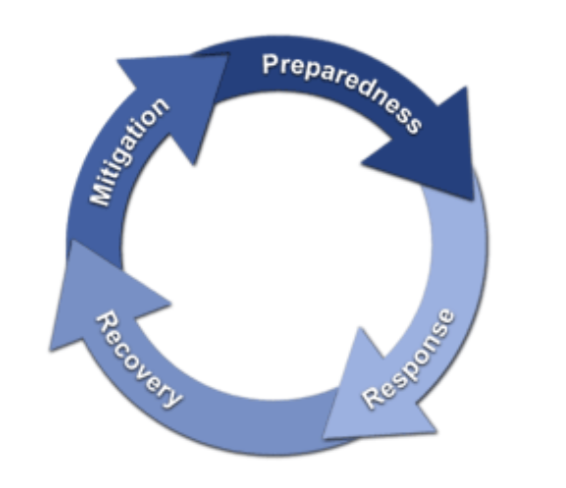
\includegraphics[scale=0.8]{ScenarioApplicativo/disaster_phase.png}
	\caption{Ciclo di fasi per il disaster-management}
	\label{fig:contesto_cycle}
\end{figure}
 \newpage
 Le definizioni di queste fasi sono svariate e variano a seconda dell'agenzia che le fornisce; a grandi linee possono essere così descritte \cite{FASI_MANAGEMENT}:
 \begin{itemize}
 \item \textbf{Mitigation:} Include tutte quelle attività svolte per ridurre le perdite di vite e proprietà a causa di un disastro naturale e/o umano: \textit{"un'azione continua che riduce o elimina il rischio a lungo termine per le persone e le proprietà da pericoli naturali e dai loro effetti"}. L'attuazione di strategie di Mitigation è una parte della fase di Recovery se applicata dopo il verificarsi di un disastro.\\
Le misure di Mitigation possono essere:
\begin{itemize}
\item\textbf{Strutturali}, forniscono soluzioni tecnologiche, come l'ampliamento degli argini di un fiume.
\item\textbf{Non strutturali}, forniscono soluzione legislative, come il divieto di costruzione su terreni paludosi.
\end{itemize}
\item \textbf{Preparednes:} Ha lo scopo di preparare al meglio la comunità attraverso attività formative.\\
Questa fase è un continuo ciclo di pianificazione, organizzazione, prove e valutazioni; in questo modo l'emergency manager sarà in grado di fornire la miglior soluzione.\\
Nella fase di preparednes si sviluppano piani d'azione per gestire e contrastare i rischi e si costruiscono le risorse necessarie per attuare tali piani. Alcune misure comuni sono: 
\begin{itemize}
\item Comunicazione dei piani con terminologia e metodi comprensibili.
\item Corretta manutenzione dei servizi d'emergenza.
\item Sviluppo ed esercizio di metodi di avviso emergenza per la popolazione.
\item Creazione di rifugi e piani di evacuazione
\end{itemize}
\newpage
\item \textbf{Response:} Include la mobilitazione dei servizi di emeregenza necessari e primi interventi nell'area colpita; è probabile che includano una prima ondata di servizi base come pompieri, polizia e ambulanze. \\
In particolare in questa fase si attuano i piani precedentemente ideati nella fase di preparednes e le attività dovrebbero includere:
\begin{itemize}
\item Ricerca e soccorso.
\item Distribuire viveri e medicinali
\item Valutazione dei danni
\item Riparo per le vittime
\item Estinzione di eventuali incendi
\end{itemize}
\item \textbf{Recovery:} Include tutte quelle attività che hanno l'obiettivo di riportare le persone alla loro "normalità". Riparazione, sostituzione e ricostruzione sono esempi tipici.\\
Lo scopo della fase di Recovery è appunto ripristinare l'area colpita allo stato precedente la catastrofe, tuttavia le azioni devono essere eseguite soltanto quando i bisogni della comunità sono stati soddisfatti e la fase di Response è quindi terminata; a quel punto si possono avviare le attività di ripristino con lo sforzo di "ricostruire indietro meglio", cioè provando a ridurre i rischi, precedenti al disastro, presenti nella comunità e nelle infrastrutture.\\
La fase di Recovery può essere divisa in due periodi. La fase a breve termine, in genere, dura da sei mesi almeno ad un anno e prevede la fornitura di servizi immediati alle imprese. La fase a lungo termine, che può durare anche decenni, richiede una pianificazione strategica efficente per affrontare gli impatti più gravi e permanenti di un disastro. \\
Le comunità devono accedere e distribuire una vasta gamma di risorse pubbliche e private per consentire la ripresa economica a lungo termine.
\end{itemize}
Un utilizzo ottimale di questo framework è in grado di fornire alla comunità le risorse necessarie affinché un disastro possa essere affrontato in maniera efficace, o meglio, si possono ridurre tutte quelle morti causate dalla negligenza di "involucri organici", privi di qualsiasi etica e morale erroneamente chiamati professionisti.
\newpage


\section{I luoghi comuni sui disastri}
Se ci venisse chiesto di immaginare lo scenario immediato ad un disastro ambientale o umano, nella maggior parte dei casi, potremmo scrivere una buona trama per un film apocalittico. Questo succede a causa di alcuni luoghi comuni diffusi nella nostra società \cite{COMMON}, ciò che ci sembra ovvio infatti potrebbe essere soltanto un mito inculcato nella nostra mente:
\begin{enumerate}
\item\textbf{ I disastri sono eventi rari}, sono una parte normale della vita quotidiana e in molti casi sono eventi ripetitivi.
\item\textbf{ I disastri naturali sono inevitabilmente il risultato della furia di madre natura}, le cause di questi eventi sono sì naturali, infatti non possiamo fare niente per eliminare i terremoti, le inondazioni o le tempeste tropicali. Tuttavia, il disastro è quasi sempre causato dalle persone e dalle comunità stesse che si mettendo in condizioni di rischio e non vi è nulla di molto naturale o inevitabile in tutto questo. 
\item\textbf{ I disastri provocano una grande quantità di caos e non possono essere gestiti in modo sistematico}, ci sono ottimi modelli teorici su come disastri funzionano e come gestirli. Dopo più di 75 anni di ricerca nel campo, gli elementi generali del disastro sono ben noti, e tendono a ripetersi da un disastro all'altro.
\item\textbf{ I disastri uccidono le persone indipendetemente dal loro status sociale o economico }, le persone povere ed emarginate sono molto più a rischio di morte di quelle ricche e benestanti.
\item\textbf{ I terremoti sono comunemente responsabili di bilanci molto elevati di morte.}, gli edifici che crollano sono i veri responsabili. Come già detto non è possibile fermare i terremoti, è possibile però costruire edifici antisismici e organizzare attività umane in modo tale da minimizzare il rischio di morte.
\item\textbf{Quando avviene il disastro il panico è la reazione più comune}, la maggior parte delle persone mantiene un comportamento razionale. Il panico non è comunque da escludere.
\item\textbf{Un gran numero di persone fuggirà dall'area colpita}, di solito c'è un "reazione di convergenza" e la zona si riempie di persone. Alcuni dei sopravvissuti se ne andranno, altri saranno evecuati ma durerà comunque poco.
\item\textbf{Dopo il disastro i sopravvissuti tendono ad essere storditi e apatici}, i sopravvissuti tendono a mettersi al lavoro per "ripulire". L'attivismo è molto più comune della rassegnazione (questa è la cosiddetta "comunità terapeutica"). Nel peggiore dei casi solo il 15-30 per cento delle vittime mostrano reazioni passive.
\item\textbf{Le persone tendono a prendere decisioni sbagliati a meno che non siano guidati dalle autorità}, le persone prendono decisioni sulla base delle informazioni che sono in grado di ottenere e di interpretare. All'interno di questa "bussola", la maggior parte del processo decisionale può essere giudicato razionale.
\item\textbf{ I disastri di solito danno luogo a diffuse manifestazioni spontanee di comportamento antisociale}, in generale i comportamenti sono caratterizzati da una grande solidarietà sociale, generosità e sacrificio di sé stessi.
\item\textbf{Il saccheggio è un fenomeno comune}, il fenomeno dei saccheggi è raro e di portata limitata. Si verifica soprattutto quando ci sono presupposti forti, come quando una comunità è già profondamente divisa.
\item\textbf{Le persone ricorrono alla violenza per proteggere i propri interessi}, La \textit{'comunità terapeutica'} è comune, infatti le persone hanno una maggiore tendenza ad aiutarsi a vicenda in situazioni d'emergenza che in tempi normali.
\item\textbf{La legge marziale deve essere imposta dopo il disastro al fine di evitare che la società si rompa del tutto}, L'imposizione della legge marziale dopo il disastro è estremamente raro, ad ogni modo il suo utilizzo implica che i normali meccanismi di governo non sono mai stati efficaci.
\item\textbf{I cadeveri non seppelliti costituiscono un pericolo per la salute}, Nemmeno la decomposizione costituisce un significativo rischio per la salute. Seppelire in modo avventato demoralizza i sopravvissuti e sconvolge le modalità di certificazione di morte, i riti funebri, e, ove necessario, l'autopsia.
\item\textbf{Le epidemie sono risultati quasi inevitabili delle distruzioni e delle scarse condizioni salutari causate dalla maggior parte dei disastri }, in generale, il livello di sorveglianza epidemiologica e l'assistenza sanitaria nella zona del disastro è sufficiente per fermare ogni possibile epidemia. Tuttavia, il tasso di diagnosi di malattie può aumentare con una migliore assistenza sanitaria, sopratutto in aree molto povere.
 \item\textbf{Una grande quantità e assortimento di medicinali dovrebbe essere inviato},  gli ospedali da campo sono solitamente installati troppo tardi per curare i feriti, finiscono per fornire assistenza generale e continuità delle cure. Poiché il trasporto e il funzionamento di questi tende ad essere costoso e logisticamente impegnativo, in alcuni casi può essere più efficiente per tentare di ripristinare o aumentare ospedali esistenti nel settore, anche se sono significativamente danneggiati.
 \item\textbf{A seguito di un disastro la vaccinazione di massa è un ottima strategia per fermare la diffusione di malattie},  considerando che la vaccinazione mirata di gruppi specifici (ad esempio, bambini, medici e infermieri) può essere una strategia efficace, la vaccinazione di massa indiscriminata è invece uno spreco.
 \item\textbf{I cadaveri, i sopravvissuti, strade, macerie e altre cose devono essere irrorati con un disinfettante per fermare la diffusione della malattia}, questa misura comune e popolare spreca grandi quantità di disinfettante e non fa assolutamente nulla per la salute pubblica.
 \item\textbf{Di solito c'è una carenza di risorse quando si verifica un disastro e questo impedisce di gestirlo in modo efficace}, le carenze se si verificano, sono quasi sempre molto provvisorie. In realtà ci sono più problemi nella buona distribuzione e utilizzo in modo efficiente rispetto all'acquisto vero e proprio.
\item\textbf{Qualsiasi tipo di aiuto è utile dopo il disastro purché sia fornito abbastanza rapidamente}, iniziative avventate e frettolose tendono a creare il caos. Inoltre saranno necessari solo alcuni tipi di assistenza tecnica, beni e servizi; infatti non tutte le risorse utili preesistenti il disastro saranno distrutti. La donazione di materiali inutilizzabili o manodopera consuma risorse di organizzazione e di alloggio che potrebbero più proficuamente essere utilizzate per ridurre il bilancio del disastro.
\item\textbf{Al fine di gestire al meglio un disastro è necessario accettare qualsiasi aiuto venga offerto}, è molto meglio limitarsi ad accettare donazioni di beni e servizi che sono effettivamente necessari nella zona del disastro.
\item\textbf{C'è un fenomeno noto come "terremoto tempo"}, la credenza popolare che i terremoti si verifichino quando vi è un clima afoso non ha alcuna base di fatto. Numerosi studi scientifici hanno cercato di individuare le condizioni atmosferiche precursorie ad un terremoto, ma l'unica osservazione riguarda il rilascio di alogeni nell'atmosfera.
\item\textbf{Gli animali sono in grado di percepire il terremoto prima che accada}, in realtà gli animali si comportano in modo insolito prima di un terremoto, tuttavia non è un modo affidabile di sapere se tale fenomeno sta per accadere.
\item\textbf{Siamo ben organizzati ad affrontare una pandemia o un attacco nucleare}, nella maggior parte dei paesi, compresi quelli più ricchi e più grandi, la fase di Preparedness è quella più trascurata e carente.
\item\textbf{In caso di un attacco terroristico biologico siamo in grado di confinare l'epidemia in modo efficace}, le scorte di anticorpi e vaccini sono insufficienti così come, i reparti di isolamento, le unità di risposta sul campo, le unità di decontaminazione, e la formazione per i soccorritori e medici. Inoltre potrebbe anche essere difficile da individuazione tempestivamente l'agente patogeno o la tossina in questione.
\item\textbf{Il panico e comportamenti irrazionali sono inevitabili conseguenze di un attacco terroristico nucleare}, in disastri di ogni genere maggior parte delle persone si sforzano di comportarsi razionalmente e prendere decisioni razionali . Questo è antitetica al panico. Tuttavia, se le persone non hanno informazioni adeguate, il loro processo decisionale può sottrarsi all'analisi razionale.
\item\textbf{I soccorritori non si presenterebbero in caso di disastro, poiché impegnati a proteggere la propria famiglia}, non è comune l'assenteismo di massa tra i soccorritori. In generale, le persone tendono ad avere un maggiore senso del dovere.
\item\textbf{I disastri accadono sempre a qualcun altro}, la sindrome dell' invulnerabilità personale, induce erroneamente le persone a ritenere che siano in qualche modo immune da disastri. Non è così.
\item\textbf{Scorte di sangue ed emoderivati devono essere inviati nei paesi stranieri colpiti}, ci sono ragioni patologiche e logistiche per le quali è meglio acquisire sangue ed emoderivati da donatori dello stesso paese colpito.
\item\textbf{Quando si verificano disastri gli adulti normodotati dovrebbero volontariamente aiutare }, l'era del volontariato spontaneo è finita. I volontari non organizzati portano più problemi di quanti ne risolvino. La risposta è quella di creare, in tempi di pace, associazioni di volontari addestrati ed equipaggiati, che possano essere integrati nel sistema di protezione civile per legge o secondo regole ben definite che definiscono i propri compiti e responsabilità.
\item\textbf{Vittime della carestia di solito muoiono di fame}, il più delle volte muoiono a causa di effetti colleterali della carestia, come la malnutrizione, diarrea, il tifo o il colera.
\item\textbf{Solo la preparazione porta ad agire}, produrre i mezzi per ridurre il rischio di catastrofi (un sistema di allarme, una mappa di pericolosità, un avanzamento delle tecniche costruttive antisismiche, di un regolamento edilizio aggiornato, ecc), non implica che verranno utilizzati; infatti la mancanza di leadership, cattive intenzioni, paralisi politica e la mancanza di fondi sono alcune possibili ragioni per cui questi mezzi potrebbero non essere utilizzati.

\end{enumerate}
\newpage

\section{Il contesto d'uso}
\label{contesto}
Il contesto d'uso è la prima parte della fase di \textit{Response }(vedi \ref{fasi}) del disaster-management cycle, nello specifico il sistema è stato progettato per essere utilizzato nei primi momenti successivi a un disastro. \\
\begin{figure}[H]
	\centering
	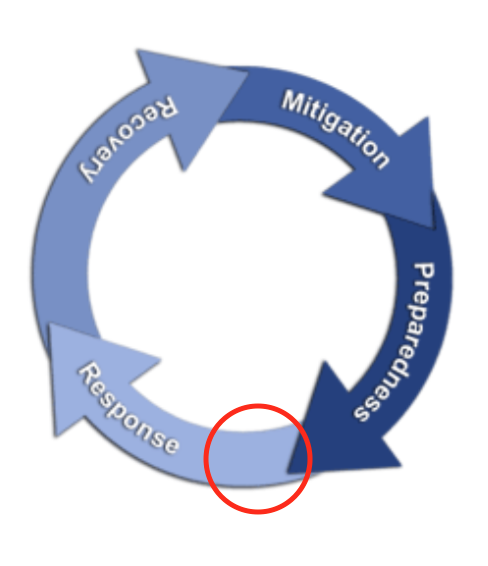
\includegraphics[scale=0.8]{ScenarioApplicativo/contesto.png}
	\caption{Contesto d'uso all'interno del disaster-management cycle}
	\label{fig:cycle_management}
\end{figure}
 \newpage
Raccogliendo alcune testimonianze sul terremoto che colpì l'Aquila nel 2009, si è individuato un fenomeno comune nel disaster management.\\
I soccorritori, sopratutto quelli non locali, ebbero difficoltà a raggiungere le vittime e fornire loro assistenza. Infatti un evento come il terremoto può modificare profondamente la topografia di intere regioni, questi cambiamenti rendono i sistemi GPS-based obsoleti. Ad esempio il cedimento del manto stradale di una certa strada potrebbe renderla impercorribile; un sistema come il navigatore potrebbe indicare ad una squadra di soccorsi un percorso che comprende tale strada, per quest'ultimi non c'è modo di sapere a priori se quel percorso è percorribile se non attraversandola metro dopo metro. \\
In queste situazioni la presenza di un sistema multiagente \cite{RESPONSE} costituisce un valido aiuto a chi gestisce l'emergenza, permettendo di avere dati aggiornabili e dinamici, prodotti dagli "agenti" (umani e non) direttamente sul campo. \\
Il lavoro di questa tesi è quindi la progettazione e lo sviluppo di un'applicazione mobile geolocalizzata con i seguenti main goals:
\begin{itemize}
\item Segnalare la posizione di un'emergenza
\item Visualizzare sulla mappa lo stato generale dell'area colpita e dei luoghi d'interesse  
\item Visualizzare lo status dei propri famigliari
\item Interagire con un sistema centrale multiagente
\end{itemize}
Nel contesto d'uso la rete è congestionata/assente, quindi è importante installare l'applicazione in tempi di pace; inoltre pur avendo un'interfaccia usabile, alcuni utenti con scarsa conoscenza nell'uso dei dispositivi mobili potrebbero dover essere istruiti. Queste attivita sono tipiche della fase di preparedness (vedi \ref{fasi}).\\
Non possiamo eliminare del tutto il \textit{Pericolo} di un disastro, tuttavia possiamo fornire uno strumento utile ad aumentare la \textit{Resilienza} (vedi \ref{vuln}) della comunità, di conseguenza diminuire il \textit{Rischio} e l'impatto di un disastro, ergo le vittime.\\
\newpage



\chapter{OpenStreetMap}
\label{cap:OpenStreetMap}
In questo capitolo si illustra brevemete il progetto OpenStreetMap, vengono sollevate alcune questioni etiche nella scelta di un map-provider e infine si espongono i motivi tecnici che hanno portato a scegliere OSM come map-provider per l'applicazione sviluppata nell'ambito di questa tesi.
\section{Cos'è OpenStreetMap ?}
OpenStreetMap (OSM) è \textbf {un progetto cartografico collaborativo, nato per creare una mappa mondiale gratuita e libera}. Gli utenti iscritti possono visualizzare, aggiungere e modificare in ogni momento la mappa, secondo un approccio analogo a quello di Wikipedia. I dati infatti sono distribuiti sotto la licenza ODbl\cite{LICENZA_OSM}: \textit{"Sei libero di copiare, distribuire, trasmettere e adattare i nostri dati, finchè lo attribuisci a OpenStreetMap e ai suoi contributori. Se alteri o ti basi sui nostri dati, puoi distribuire il risultato sotto la stessa licenza [...]"}.\\
\begin{figure}[H]
	\centering
	
\includegraphics[scale=0.1]{OpenStreetMap/logo.png}
	\caption{Il logo di OpenStreetMap}
	\label{fig:logo_OSM}
\end{figure}
Si potrebbe erroneamente pensare che l'esistenza di una mappa gratuita non sia una novità; in realtà  i dati geografici \cite{MAPPE_LIBERE}, nella gran parte del mondo (Italia ed Europa incluse), non sono gratuiti. In linea di massima l'onere della realizzazione di mappe è delegata ad agenzie nazionali che poi le rivendono a privati o aziende e ne ricavano finanziamenti. Gli Stati Uniti d'America sono l'unica eccezione macroscopica: qui, infatti, le leggi sul copyright delle agenzie nazionali rendono questi dati di pubblico dominio.\\
In altre parole se si vive in uno di questi paesi, si pagano le tasse perché vengano realizzate le mappe e si paga nuovamente per avere copie di esse o meglio "fotocopie". Di fatto si tratta di vere e proprie fotocopie poiché non possono essere modificate, sebbene spesso le mappe contengano errori intenzionali (chiamati in gergo easter eggs). Si tratta solitamente di strade inesistenti o mancanti, oppure indicazione di edifici che in realtà non esistono. Se si tenta di realizzare una mappa partendo da questi dati, le ditte od enti che le hanno realizzate potranno dire di avervi beccato semplicemente controllando se sono presenti i loro errori.\\
La comunità di OSM è in forte crescita: dal 2004, anno in cui nasce da un'idea di Steve Coast ,ad oggi, il numero di utenti iscritti e i loro contributi sono cresciuti anno dopo anno, come illustrato in Figura 1.2 .
\begin{figure}[H]
	\centering
	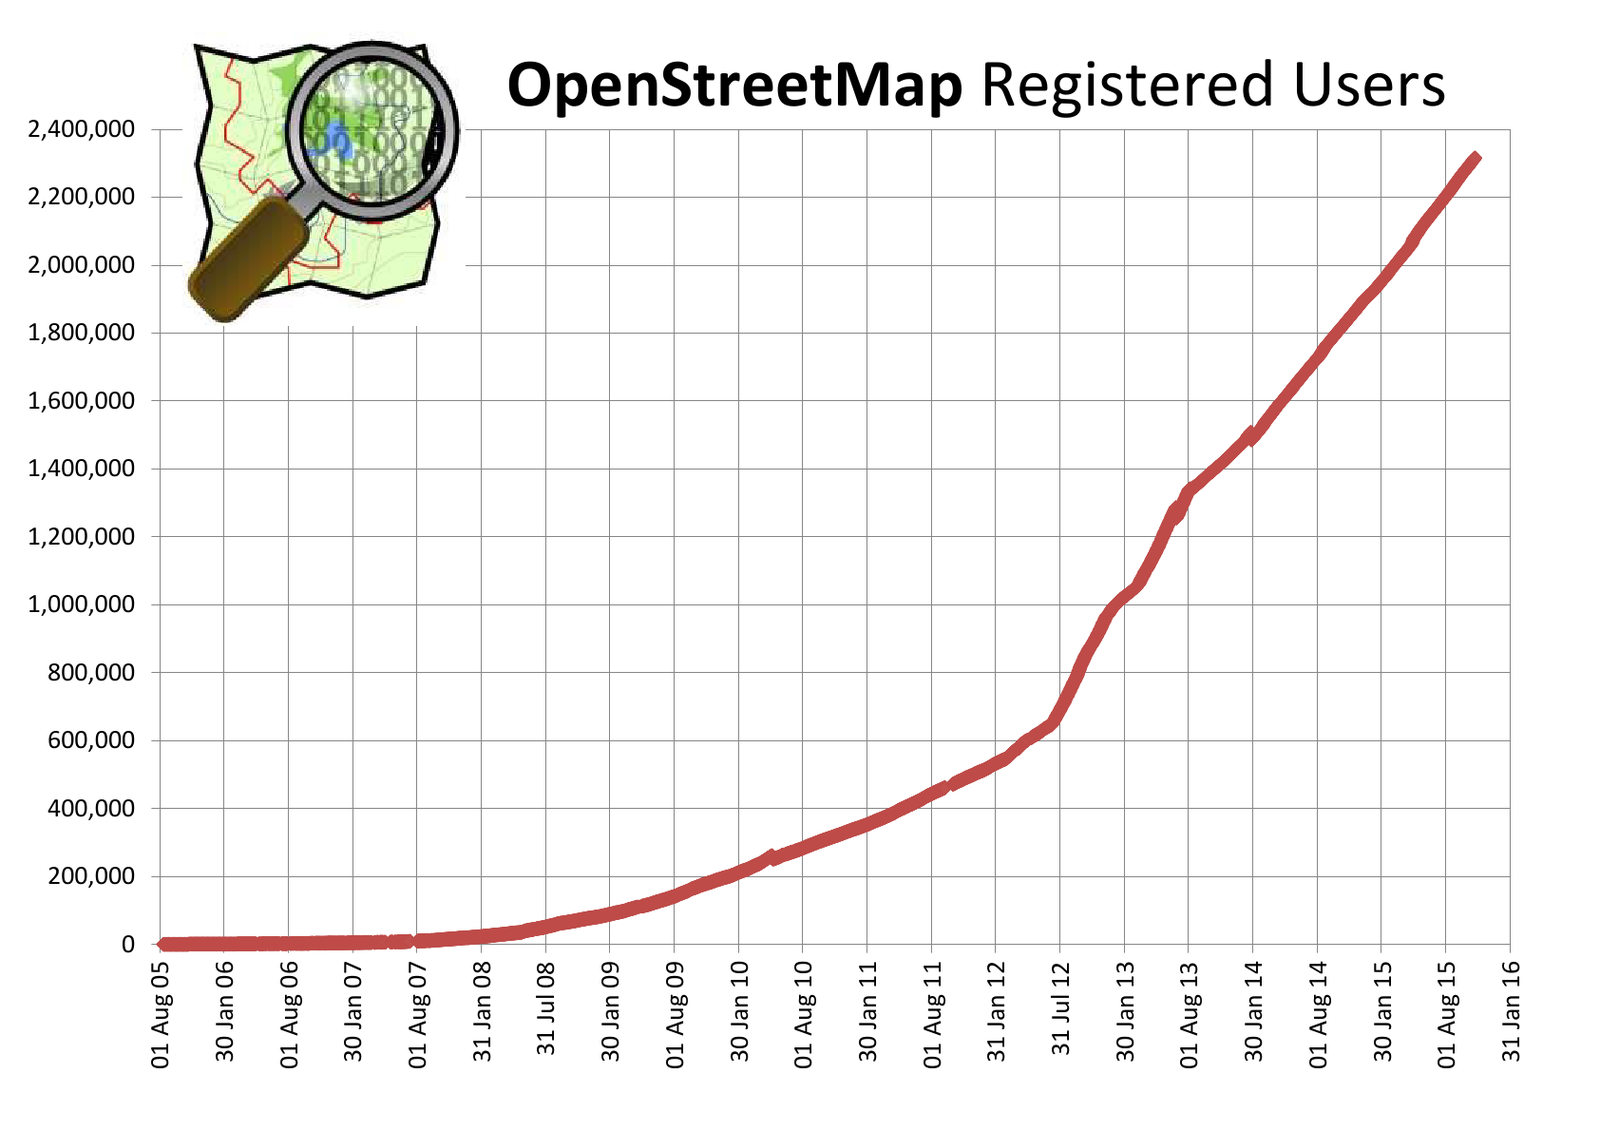
\includegraphics[scale=0.5]{OpenStreetMap/utenti.png}
	\caption{Scala lineare di utenti iscritti ad OpenStreetMap}
	\label{fig:utenti_OSM}
\end{figure}
Nel prossimo paragrafo si illustreranno meglio i motivi dell'esistenza di un progetto come OSM.


\newpage 
\section{Perchè il mondo ha bisogno di OSM} 

Finora quello di OSM sembrerebbe un altro progetto di nobile causa ma fine a se stesso. Per comprendere meglio la sua importanza bisogna fare un passo indietro nella storia e tornare nel 1800 \cite{WHYNEED} .\\
In quel periodo uno dei tanti problemi era costituito dal tempo, non in termini di tempo a disposizione, ma di che ora fosse. Gli orologi esistevano già, ma ogni città aveva il suo "tempo locale". Viene da sé come anche prendere un banale appuntamento con l'amico del paese vicino, comportasse una grande difficoltà. Successivamente l'adozione di uno standard comune ha reso il tempo \textbf{universale, libero e di tutti}.
L'equivalente attuale del dilemma del tempo è la posizione geografica, e diversi soggetti stanno cercando di diventarne il riferimento assoluto (Google spende un miliardo di dollari l'anno per mantenere le proprie mappe). 
Dunque perché il mondo ha bisongo di OSM? La risposta è semplice, perché in una società nessuna azienda dovrebbe avere il monopolio su qualcosa. I luoghi sono un bene comune, e dando ad una o poche entità questo potere gli viene dato non solo il potere di dirti la tua posizione, ma anche di poterla manipolare.
Ci sono tre aspetti da analizzare:
\begin{itemize}
\item Cosa viene visualizzato
\item Dove dovresti andare
\item Privacy personale\\
\end{itemize} 

\textbf{Cosa viene visualizzato:} Chi decide cosa debba essere visualizzato su una mappa di Google? Ovviamente Google. Se pensiamo ad un servizio pubblico, questo deve essere il più imparziale e trasparente possibile, come potrebbe esserlo se utilizza un mappa di Google?.\\
Il punto è, nel momento in cui si sceglie un provider di mappe, gli viene dato il potere di decidere quali siano gli elementi a cui dare risalto, o quali non debbano essere proprio mostrati.\\\\
\textbf{Dove dovresti andare:} La seconda questione riguarda il posizionamento. Chi decide cosa sia più vicino a me? Ancora una volta la risposta è banale. Non è un caso che scrivendo su Google Maps la parola \textit{"colazione"} vengano mostrate le grandi catene come McDonald's piuttosto che il bar sotto casa.\\
Nell'immagine successiva viene mostrato uno screenshot della ricerca \textit{"colazione"} effettuata su Google Maps all'interno della biblioteca di scienze umane dell'universita dell'Aquila. 

\begin{figure}[H]
	\centering
	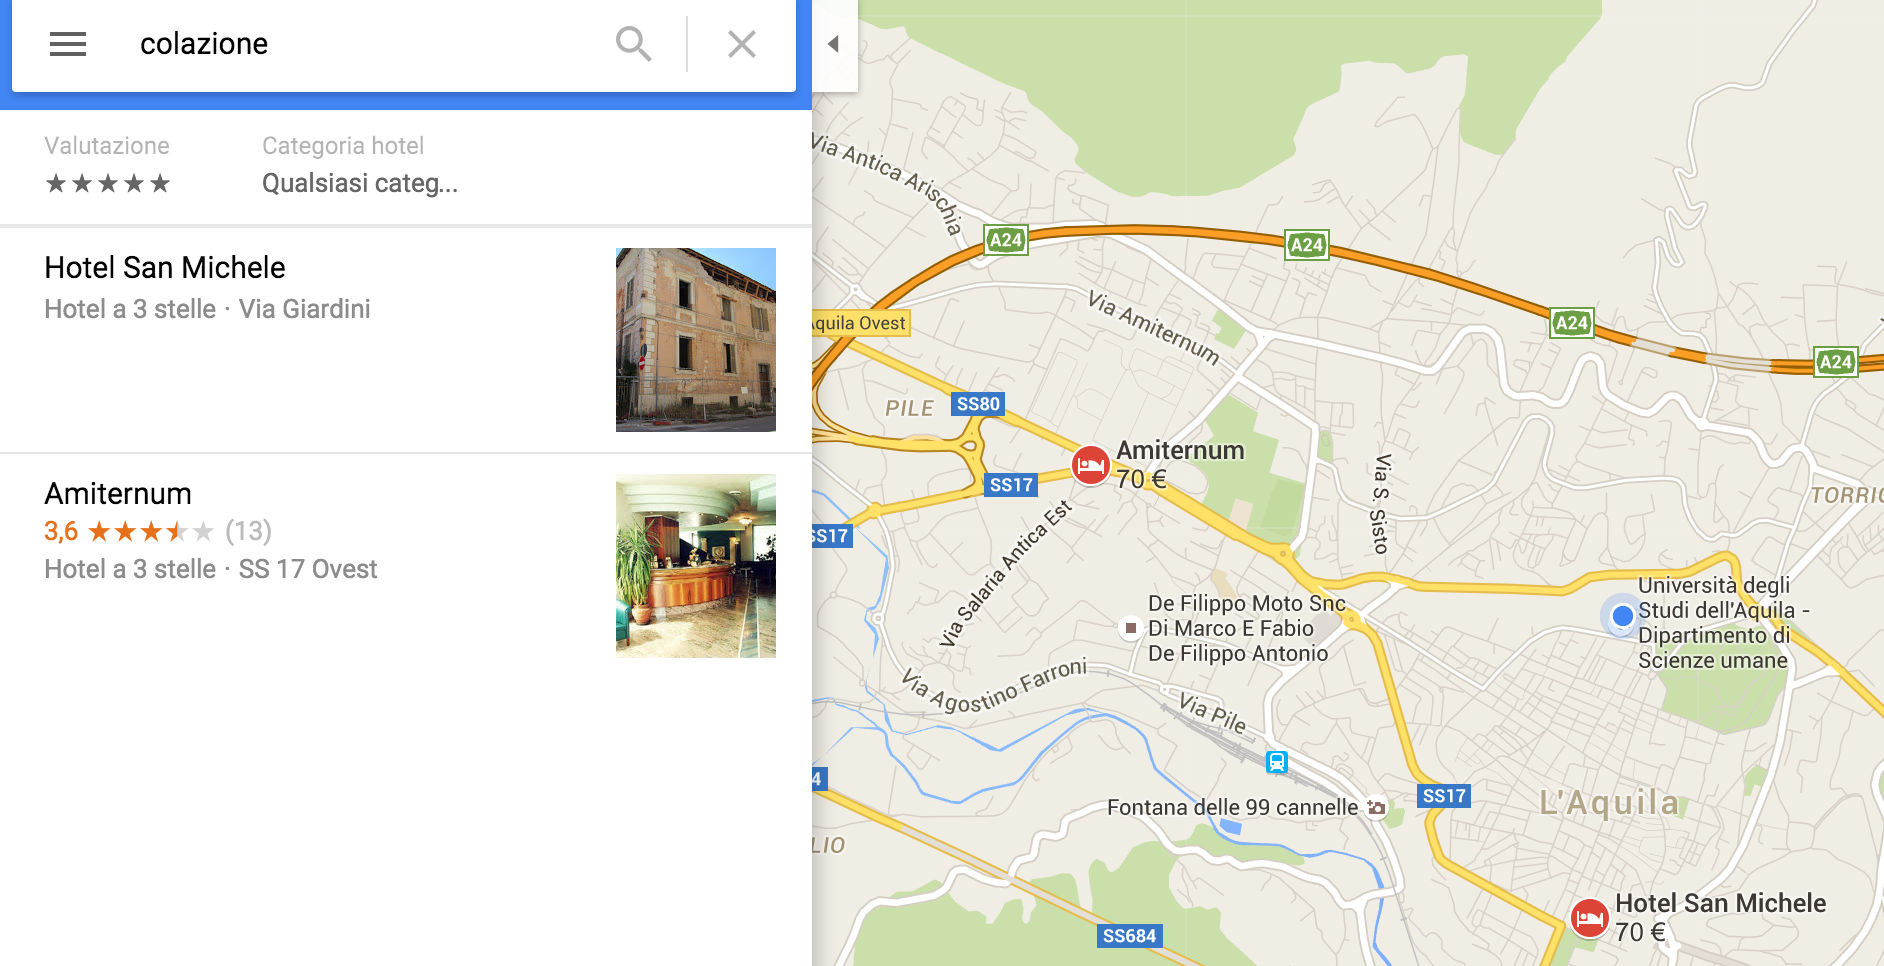
\includegraphics[scale=0.4]{OpenStreetMap/colazione.png}
	\caption{Risultato ricerca "colazione"}
	\label{fig:Ricerca_colazione}
\end{figure}

Come possiano notare vengono mostrati soltanto due hotel locali, che probabilmente hanno pagato il provider, nonostante ci sia un piccolo bar appena fuori la struttura.\\\\
\textbf{Privacy personale:} L'ultima questione riguarda la privacy. Sia Google che Apple raccolgono una quantita smisurata di informazioni sulla posizione degli utenti che utilizzano le loro API. E’ evidente che non si possono ignorare le implicazioni sociali che comporta la disponibilità di così tanti dati in mano ad una singola azienda, indipendentemente da quanto si dichiari benevola.  Aziende come Foursquare utilizzano il mezzo della “gamification” per coprire quello che di fatto è un’opera di acquisizione di dati, e anche Google è entrata nella partita della “gamification” con \textit{Ingress}, un gioco che sovrappone un mondo virtuale a quello reale e porta gli utenti a raccogliere foto e informazioni stradali con l’obiettivo di combattere, o favorire, un’invasione aliena.



\newpage
\section{OpenStreetMap vs Google Maps}
Tralasciando le questioni etiche e al fine della realizzazione dell'applicazione, sono stati analizzati i seguenti topic per la scelta del map-provider:
\begin{itemize}
\item Accuratezza
\item Costo e Download
\item Scalabilità\\
\end{itemize} 

\textbf{Accuratezza:} Poiché le mappe fornite da OSM sono il frutto di lavori "amatoriali", si è indotti a pensare che queste non rispecchino la realtà. Come in ogni progetto in stile wiki, non c'è alcuna garanzia riguardo l'accuratezza dei dati. C'è da dire, però, che quasi nessuna mappa "commerciale" dà alcuna garanzia di accuratezza. In fondo, gli errori intenzionali, sono per l'appunto, errori. \cite{ACCURATEZZA_MAPPE} \\
L'essenza stessa dei processi in stile wiki è che gli utenti stessi, tutti gli utenti, hanno un ruolo nell'accuratezza dei contenuti. Se qualcuno dovesse inserire dati errati, per errore o con intenzione, tutti gli altri possono accorgersene e correggere l'errore o semplicemente eliminarlo. La presenza di una larghissima maggioranza di utenti benintenzionati garantisce che gli errori restino entro un limite accettabile.\\
L'esperienza degli altri progetti basati su wiki ci insegna, comunque, quanto sia agevole raccogliere dati di buona/ottima qualità e quanto, invece, possa essere complicato scovare gli inevitabili errori.
Attualmente non sono stati realizzati processi o meccanismi che rendano semplice questo genere di controllo, tuttavia una comunità attiva come quella di OSM garantisce un controllo qualità sufficiente.\\
La domanda che dobbiamo porci è chi meglio di noi conosce il quartiere dove abitiamo? O la strada che percorriamo tutti i giorni o il parco dove portiamo il nostro animale a passeggiare? La risposta è \textbf{NOI}. Ed è proprio questo sottile concetto a fare la differenza tra una mappa OSM e una mappa proprietaria.\\
Utilizzando uno dei tanti "map-compare" sulla rete possiamo fare degli esempi concreti. Nella Figura 1.4 abbiamo una duplice visualizzazione dell'area universitaria di Coppito (L'Aquila): a sinistra vediamo la mappa ottenuta tramite dati OSM mentre a destra la stessa mappa fornita da Google.

\begin{figure}[H]
	\centering
	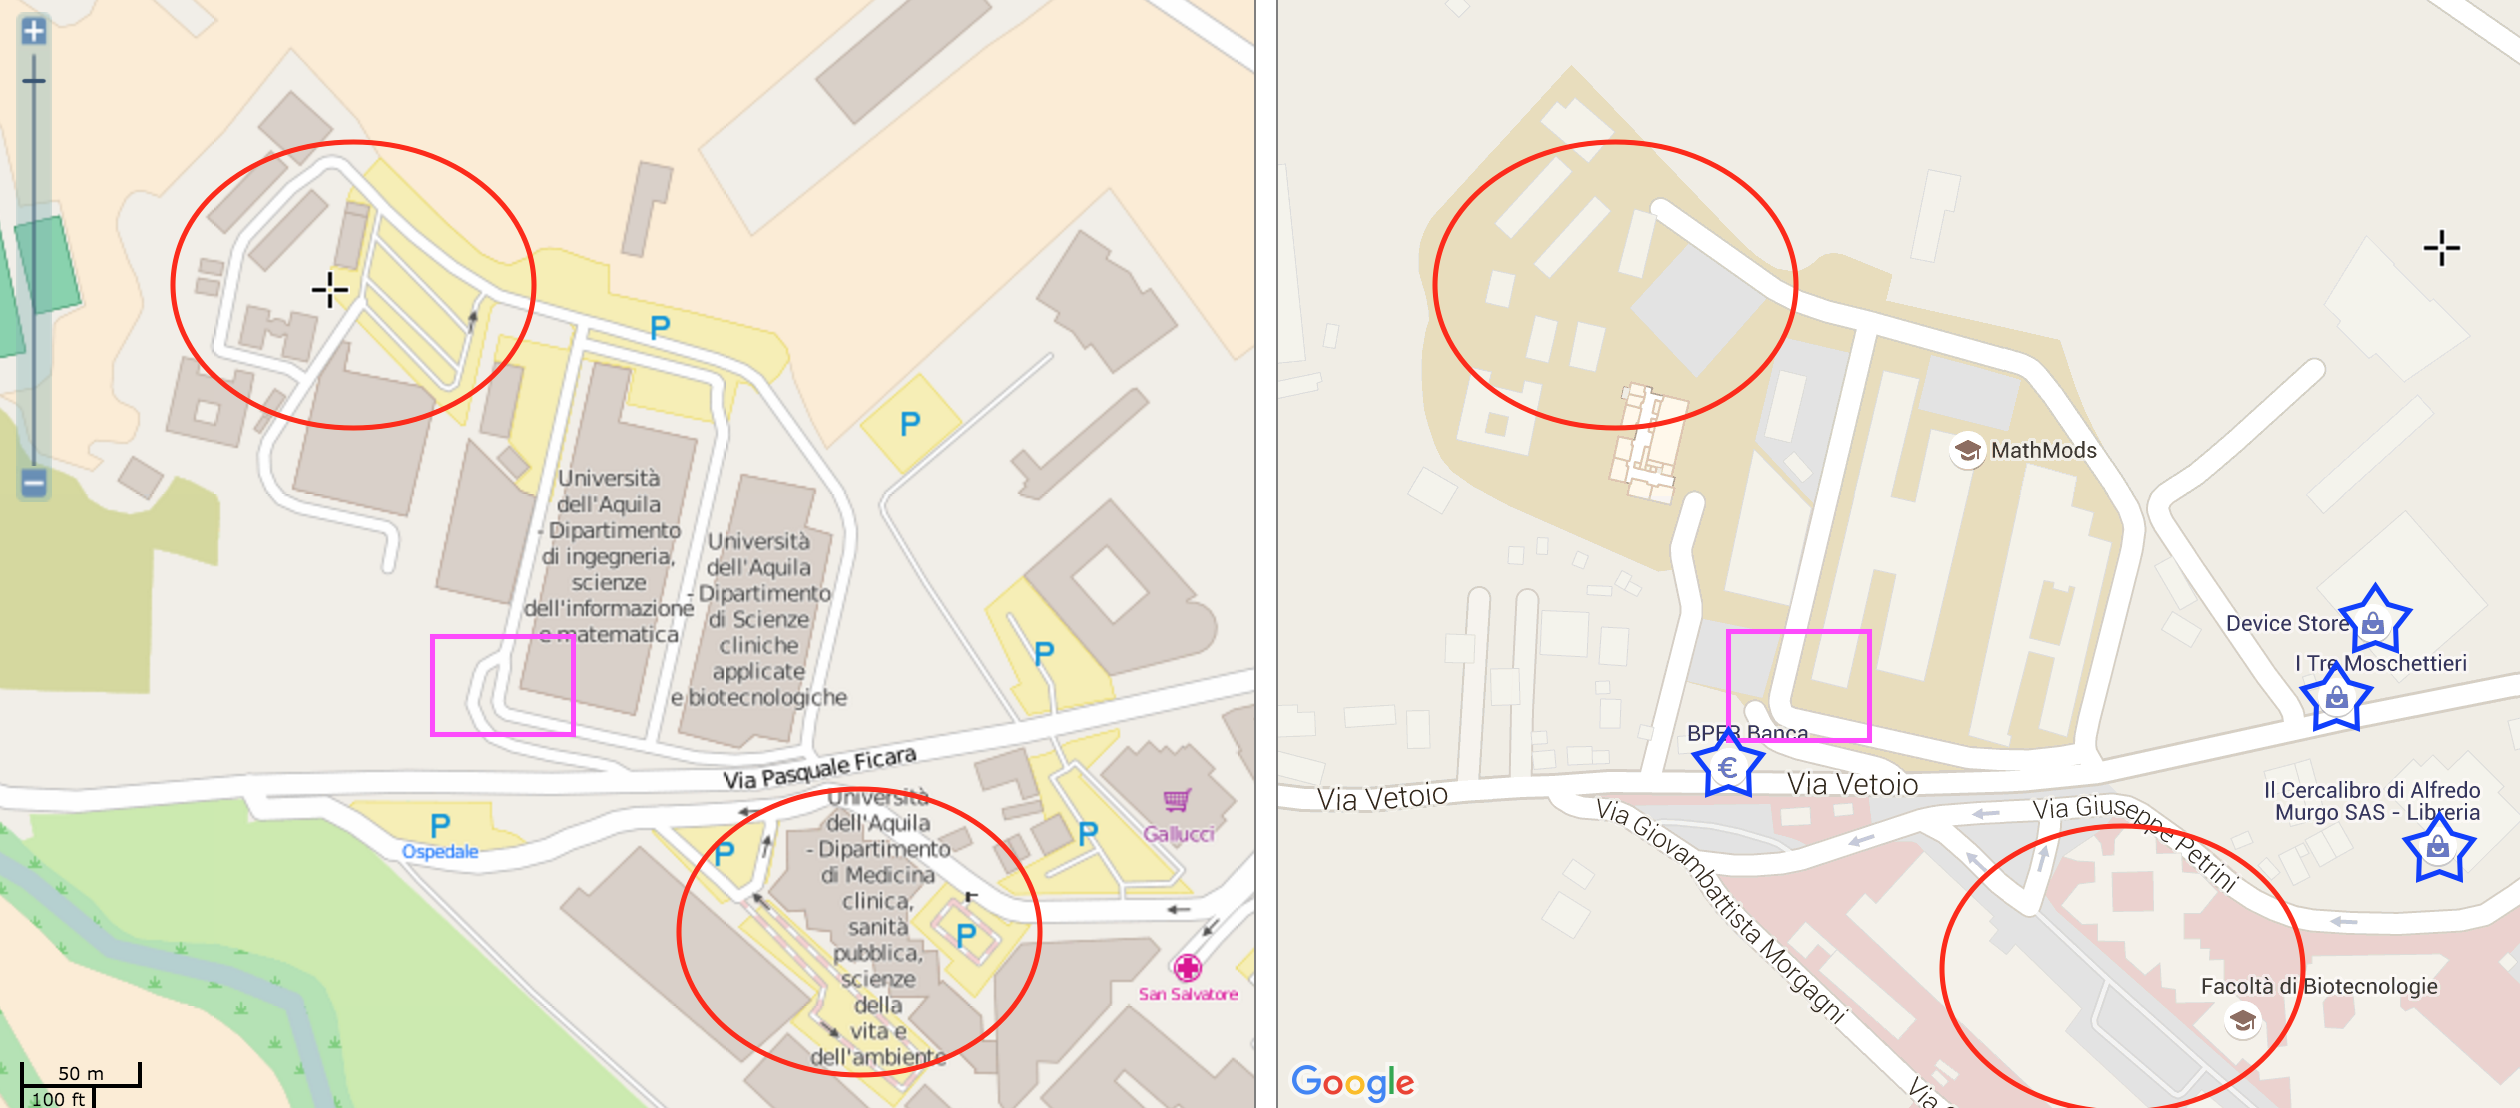
\includegraphics[scale=0.3]{OpenStreetMap/map_compare_coppito.png}
	\caption{Polo universitario di Coppito-L'Aquila}
	\label{fig:Compare_Coppito}
\end{figure}

Soffermiamoci quindi soltanto sulle porzioni di mappa racchiuse nelle diverse figure geometriche:

\begin{itemize}
\item \textbf{Cerchi rossi:} notiamo come nella mappa di Google siano assenti diverse strade interne alla struttura che collegano i diversi edifici tra di loro; questi sono percorribili da un veicolo d'emergenza o più semplicemente un'autovettura.
\item \textbf{Rettangolo viola:} Presenza di un errore (possibile easter eggs) da parte di Google: la strada non si interrompe in quel modo
\item \textbf{Stelle blu:} Presenti solo nella mappa di Google, indicano tutte attività commerciali, sarà un caso?
\end{itemize} 

Infine osservando la mappa fornita da Google non si percepisce di avere davanti una grande struttura universitaria, mentre sulla mappa OSM sono indicati perfino i nomi dei dipartimenti presenti nei diversi edifici. \newpage

\textbf{Costo e download:} Volendo realizzare un'applicazione per dispositivi mobili completamente gratuita, priva di pubblicità o di qualsiasi atra forma di lucro, di questo fattore non si può non tenere conto.
Per quanto riguarda Google, l'API javascript è gratis fino ad un massimo di venticinquemila richieste giornaliere per novanta giorni consecutivi. Superata questa soglia si ha un costo di \$ 0,50 ogni mille richieste \cite{GOOGLE_PLAN}. \\
Oltre al costo vengono applicate le seguenti restrizioni:

\begin{itemize}
\item \textbf{Area limitata:} è possibile scaricare una porzione di mappa la cui dimensione massima non superi i centoventimila chilometri quadrati              \cite{GOOGLE_OFFLINE}.
\item \textbf{Scadenza:} le mappe saranno disponibili in assenza di rete per un totale di 30 giorni, dopodiché si dovrà effettuare l'accesso alla rete.
\end{itemize}

Per quanto riguarda OSM, essendo un progetto open-data, non vi è alcuna restrizione. Infatti, è possibile scaricare l'intera mappa del mondo o porzioni di essa in totale libertà e conservarle a tempo indeterminato \cite{LINK_PLANET}.
\newpage

\textbf{Scalabilità:} Quest'ultimo topic ha segnato di fatto il punto decisivo per la scelta di OSM come map-provider. L'associazione no-profit HOT (Humanitarian Openstreetmap Team), ha lo scopo di fornire un valido supporto sul campo al mapping di aree colpite da disastri ambientali e non.\\
Nel sito ufficiale si possono visualizzare i rapporti delle principali emergenze a cui l'associazione ha partecipato \cite{HOT_PROJECT} , consideriamo quindi il terremoto di Haiti.\\
Il 12 gennaio 2010 un violento terremoto di magnitudo 7.0 Mw (quello che colpi L'Aquila nel 2009 fu di 6.3 Mw) con epicentro localizzato a circa 25 chilometri in direzione ovest-sud-ovest della città di Port-au-Prince, capitale dello Stato caraibico di Haiti, colpì tutta l'area circostante.\\
Il numero di vittime è stato stimato al 24 febbraio 2010 in 222.517. Secondo la Croce Rossa Internazionale e l'ONU, il terremoto avrebbe coinvolto più di 3 milioni di persone \cite{WIKI_HAITI}.\\ Sei ore dopo il disastro la mappa disponibile di Port-au-Prince era la seguente:

\begin{figure}[H]
	\centering
	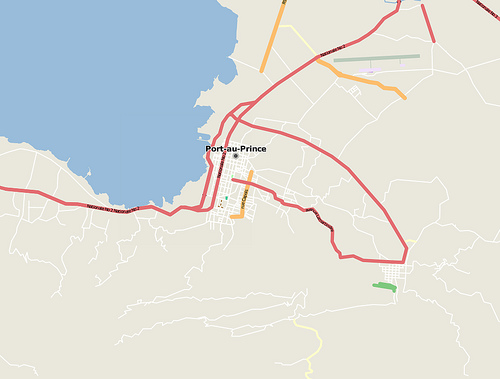
\includegraphics[scale=0.6]{OpenStreetMap/haiti_prima.jpg}
	\caption{Mappa OSM di Pourt-au-Prince 6 ore dopo il terremoto del 2010}
	\label{fig: haiti_day0}
\end{figure}
\newpage
Nelle ore successive, numerose aziende di geo-data (Geo-eye, Google, Yahooo...) resero pubbliche le proprie immagini satellitari, in modo tale che i volontari potessero mappare l'area colpita dal proprio pc in qualsiasi parte del mondo. \\
Quello che avvenne fu qualcosa di straordinario, come disse Jeffery Johnson \textit{"What we did in Haiti changed disaster response forever"}. \\
Il contributo di più di seicento volontari portò ad avere dopo appena 48h dal disastro la seguente mappa:

 \begin{figure}[H]
	\centering
	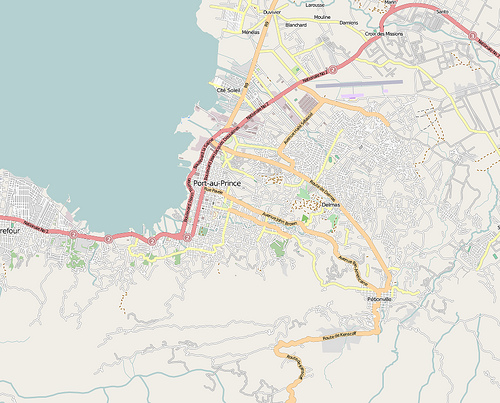
\includegraphics[scale=0.6]{OpenStreetMap/haiti_dopo.jpg}
	\caption{Mappa OSM di Pourt-au-Prince 48 ore dopo il terremoto del 2010}
	\label{fig: haiti_day2}
\end{figure}

La mappa nelle settimane successive continuò ad essere aggiornata e raffinata, tutto questo ha facilitato il coordinamento delle operazioni umanitarie di soccorso e approvigionamento, salvando di fatto innumerevoli vite.\\
In conclusione OSM garantisce un'ottima scalabilità, caratteristica che come abbiamo visto, nei contesti di disaster-management è di fondamentale importanza. 

\chapter{L'applicazione lato utente}
Nella prima parte di questo capitolo, vengono illustrati i requisiti di sistema che hanno guidato lo sviluppo dell'intera applicazione. Mentre nella parte finale verranno mostrate le schermate grafiche relative ai task principali.

\section{Requisiti di sistema}
La stesura dei requisiti di sistema è un processo imprenscindibile per la progettazione, nel nostro caso è il risultato di un processo iterativo basato sulla valutazione di un esperto.\\
I requisiti sono divisi in:
\begin{itemize}
\item \textbf{Requisiti funzionali} indicano quello che il sistema deve fare
\item \textbf{Requisiti non funzionali} vincoli sul sistema e il suo sviluppo
\end{itemize}
 
 \subsection{Requisiti funzionali}

\begin{enumerate}
\item Interazione mappa
  \begin{itemize}
     \item\textit{identificativo:} RF-1
  \item\textit{Descrizione:} Il sistema deve permettere all’utente di interagire con la mappa, compiendo le azioni basilari quali: zoom In, zoom Out, CCW (Change Center View), click.
  \end{itemize}
  
\item Impostazione POI
  \begin{itemize}
  \item\textit{identificativo:} RF-2
  \item\textit{Descrizione:} Il sistema deve permettere all’utente di impostare una specifica porzione di mappa come un POI (point of interest).
  \item\textit{ Razionale:} In questo modo l’utente può applicare un filtro sulla mappa (vedi RF-7)  e visualizzare rapidamente lo status dei luoghi d’interesse.
  \end{itemize}
  
\item Impostazione FOI
  \begin{itemize}
  \item\textit{identificativo:} RF-3
  \item\textit{Descrizione:} Il sistema deve permettere all’utente di impostare altri utenti del sistema come FOI (family of interest).
  \item\textit{ Razionale:} l’utente può in questo modo applicare un filtro (vedi RF-7) e visualizzare in modo rapido lo status delle persone d’interesse.
  \end{itemize}
  
  \item Segnalazione evento
  \begin{itemize}
  \item\textit{identificativo:} RF-4
  \item\textit{Descrizione:} l’utente deve poter segnalare la posizione di un certo evento (vedi RNF-1). 
La procedura standard di segnalazione deve avvenire sia cliccando su un punto della mappa sia tramite una schermata dedicata.
Nel caso di rete congestionata o assente il sistema deve provvedere alla bufferizzazione delle richieste e avvisare di tale situazione l’utente stesso.
  \item\textit{ Razionale:} In questo modo gli utenti contribuiscono all’aggiornamento dello status generale del territorio colpito.
  \end{itemize}
  
   \item Aggiornamento status
  \begin{itemize}
  \item\textit{identificativo:} RF-5
  \item\textit{Descrizione:} L’utente può cambiare il suo status (vedi RNF-4). Il sistema quindi deve comunicare immediatamente al server tale aggiornamento.
  \item\textit{ Razionale:} In questo modo gli utenti contribuiscono a fornire informazioni dinamiche sul territorio colpito e su se stessi.
  \end{itemize}
  
  \item Trusty data
  \begin{itemize}
  \item\textit{identificativo:} RF-6
  \item\textit{Descrizione:} Il sistema deve informare l’utente sul grado di aggiornamento delle informazioni visualizzate, ovvero:
    \begin{itemize}
    \item Eventi
    \item Status dei POI
    \item Status dei FOI
    \item mappe offline
    \end{itemize}
   L’attendibilità degli eventi è data dal numero di segnalazioni di tale evento nella relativa cella (vedi RNF-1) e dall’orario in cui è stata generata l’ultima    segnalazione.
   \item\textit{ Razionale:} Nel contesto d’uso, la rete potrebbe collassare o più semplicemente gli utenti potrebbero non utilizzare il sistema per un certo periodo, in questo modo si garantisce la totale trasparenza delle informazioni fornite.
  \end{itemize}
  
  \item Filtra mappa
  \begin{itemize}
  \item\textit{identificativo:} RF-7
  \item\textit{Descrizione:} Il sistema deve permettere all’utente di filtrare le informazioni visibili sulla mappa in base a:
    \begin{itemize}
    \item propri POI
    \item tipo eventi
    \item propri FOI
    \end{itemize}
   \item\textit{ Razionale:} La mappa visualizzata dall’utente potrebbe contenere un numero elevato di informazioni.
  \end{itemize}
  
    \item Modalità offline
  \begin{itemize}
  \item\textit{identificativo:} RF-8
  \item\textit{Descrizione:} Il sistema deve salvare porzioni di mappa visualizzate dall’utente attraverso l’interazione base (vedi RF-1) nella memoria temporale, inoltre l’utente deve poter scaricare una specifica center view su diversi livelli di zoom. Il sistema quindi deve permettere all’utente di utilizzare la modalità offline, in questo caso la rete verrà utilizzata solamente per inviare e ricevere aggiornamenti riguardo:
    \begin{itemize}
    \item POI e NPOI
    \item FOI e NFOI
    \item Eventi
    \end{itemize}
   \item\textit{ Razionale:} L’utente potrebbe voler utilizzare la modalità offline per risparmiare dati o per la  pessima connessione
  \end{itemize}
  
   \item Markercluster
  \begin{itemize}
  \item\textit{identificativo:} RF-9
  \item\textit{Descrizione:} Il sistema per livelli di zoom inferiori a 16 deve provvedere a raggruppare i marker, in un unico markerclusterer mostrando l’informazione in modo quantitativo.
  \end{itemize}
  
    \item Aggiornamento dati persistenti
  \begin{itemize}
  \item\textit{identificativo:} RF-10
  \item\textit{Descrizione:} Il sistema deve periodicamente richiedere al server l’aggiornamento dei dati persistenti (vedi RNF-2).
Inoltre l’utente può richiedere l’aggiornamento in qualsiasi momento
  \end{itemize}
  
   \item Salta a
  \begin{itemize}
  \item\textit{identificativo:} RF-11
  \item\textit{Descrizione:} Il sistema deve permettere all’utente di spostare la propria center view al NPOI (nearest point of interest), al NFOI (nearest family of interest) o al riferimento di una notifica d’allerta (vedi RF-11) cliccando su di essa.
   \item\textit{ Razionale:} L’utente potrebbe voler prestare soccorso al famigliare o visualizzare lo status del punto d’interesse più vicino a lui.
  \end{itemize}
  
   \item Notifiche di allerta
  \begin{itemize}
  \item\textit{identificativo:} RF-12
  \item\textit{Descrizione:} Il sistema deve notificare l’utente sull’aggiornamento dello status di un FOI o della segnalazione di un evento all’interno di un POI.
  \end{itemize}
  
\end{enumerate}



\chapter{L'implementazione}
In questo capitolo verranno illustrati i framework utilizzati per l'implementazione dell'applicazione e l'algoritmo ideato per la creazione di una griglia sulla mappa con il relativo codice Javascript.
\section{Le applicazioni cross-platform}
Negli ultimi anni, i dispositivi mobili sono diventati sempre più parte integrante della nostra vita, grazie al progresso tecnologico e all'abbattimento dei prezzi, oggi costituiscono un bene alla portata di tutti. \\
La possibilità di scegliere tra una vasta gamma di smartphone diversi per caratteristiche e produttore, ha reso più complicata la vita delle aziende informatiche che sono costrette a considerare l'eterogeneità dei vari sistemi operativi in circolazione.\\
\begin{figure}[H]
	\centering
	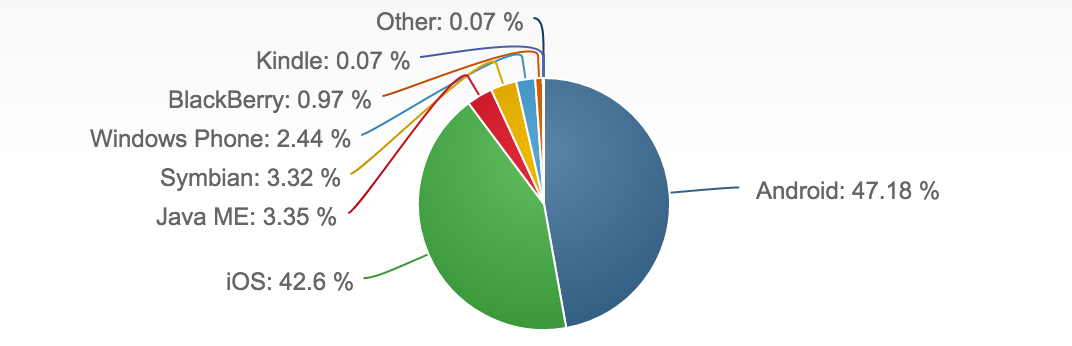
\includegraphics[scale=0.7]{Implementazione/os.png}
	\caption{Utilizzo dei vari OS su scala mondiale}
	\label{fig:os_mobile}
\end{figure}
\newpage
Chi sviluppa applicazioni mobili, può scegliere tra due approcci:
\begin{enumerate}
\item \textbf{Scegliere uno degli OS mobile} e implementare l'applicazione utilizzando il linguaggio nativo.
\item \textbf{Scegliere un framework }che, utilizzando un meta-linguaggio, sia in grado di generare diverse versioni dell'applicazione per i relativi OS.
\end{enumerate}
I diversi approcci forniscono rispettivamente pro e contro. Per il primo i vantaggi sono una maggiore velocità del sistema, la possibilità di creare un'interfaccia rispettando il look and feel nativo e pochi problemi di compatibilità. Lo svantaggio è invece legato alla \textbf{bassa portabilità}, l'applicazione andrà riscritta completamente per dispositivi con diversi OS. \\
Il principale vantaggio del secondo approccio, è invece la possibilità di riutilizzare lo stesso codice per generare varie versioni dell'applicazione per diversi OS, questo a discapito di una minore velocità del sistema se l'applicazione fosse sviluppata nel linguaggio nativo. \\
Considerando il contesto d'uso del sistema ( vedi \ref{contesto}), è chiaro che la nostra applicazione dovrebbe poter essere installata su qualsiasi dispositivo (ndr l'idea di salvare vite con un certo OS non è delle più nobili), di conseguenza si è adottato tale approccio.\\
La filosofia \textit{"Write once, run anywhere"}, non è un concetto nuovo nell'informatica, lo slogan fu ideato dalla Sun Microsystems per descrivere un linguaggio (Java) in grado di essere eseguito su diverse macchine. Nel corso degli anni diverse software-house hanno realizzato dei framework in grado di fare questa "magia", sostanzialmente ne estitono due tipi:
\begin{itemize}
\item \textbf{ I Cross-Compiling:} si scrive l'applicazione in un certo linguaggio, successivamente un framework riesce a compilarlo per le diverse piattaforme (Appcelerator Titanium1, Corona SDK2, Xamarin Monotouch3); Solitamente sono framework professionali e a pagamento.
\item \textbf{I Browser-Embedding:} più recenti, consentono di sviluppare il codice con le tecnologie del web (HTML5, CSS3, Javascript), l'applicazione verrà avviata nel dispositivo mobile all'interno di un browser (PhoneGap, Apache Cordova).
\end{itemize} 
Ancora una volta è stato scelto il secondo approccio, nello specifico il framework PhoneGap.

\section{PhoneGap}
\label{phonegap}
Phonegap è un framework di sviluppo mobile prodotto da Nitobi e acquistato successivamente da Adobe Systems. Permette ai programmatori software di creare applicazioni per dispositivi mobili utilizzando esclusivamente HMTL, CSS e Javascript invece di utilizzare linguaggi nativi come Object-C e C++. Il risultato sono applicazioni ibride, nel senso che non sono né del tutto native (perché tutto il rendering del layout è fatto tramite viste web e non tramite i framework UI delle piattaforme native) né del tutto web-application (perché non sono applicazioni solo web, ma hanno anche accesso alle funzioni interne dei device tramite le API). \\
Il software alla base di PhoneGap è \textit{Apache Cordova} ed è open source. \\
\begin{figure}[H]
	\centering
	
\includegraphics[scale=0.6]{Implementazione/logo_phonegap.png}
	\caption{Logo del framework PhoneGap}
	\label{fig:logo_phonegap}
\end{figure}
Presentato la prima volta in un evento iPhoneDevCamp a San Francisco, PhoneGap ha vinto il premio People's Choice Award alla conferenza O'Reilly Media Web nel 2009. Il framewotk PhoneGap viene utilizzato da molte piattaforme  di sviluppo software come ViziApps, Worklight, Convertico e appMobi. \\
Il 4 ottobre 2011 Adobe annuncia ufficialmente l'acquisizione della Nitobi Software. In concomitanza il codice PhoneGap ha contribuito con la Apache Software Foundation ad iniziare un nuovo preocetto chiamato Apache Cordova.
\newpage
PhoneGap non è altro che un modulo software che permette agli sviluppatori di incorporare le loro applicazioni web all'interno di applicazioni native di diverse piattaforme. Le applicazioni che utilizzano questo framework sono scritte in HTML5, CSS3 e Javascript e il collegamento con le livrerie native, specifiche di ogni piattaforma, è fatto tramite le API che mette a disposizione il framework.
PhoneGap fa quindi da ponte tra il sistema operativo e la web application realizzata dallo sviluppatore. Indipndentemente dalla piattaforma sottostante esisterà un modo per invocare le API native mediante funzioni Javascript. \\
Il programmatore quindi utilizzerà le API fornite da PhoneGap per accedere alle risorse hardware e software del device in modo da aggiungere le funzionalità di base al motore JAvascript e renderle facilmente utilizzabili come se fossere vere e propri metodi di una libreria. Dopo la compilazione, che avviene tramite il servizio cloud \textbf{PhoneGap Build} (Figura \ref{fig:phonegap_build}), viene generato un pacchetto internamente composto da due elementi principali con differenti responsabilità che però cooperano tra loro per fornire delle funzioni a valore aggiunto. In pratica esiste un runtime basato su WebKit4 in cui vengono iniettate le componenti statiche; il risultato sarà un pacchetto composta da due elementi principali con differenti responsabilità che però cooperano tra loro per fornire delle funzioni a valore aggiunto. Nel caso specifico il runtime si occupa di dialogare direttamente con il dispositivo e le parti statiche offrono l'interfaccia verso l'utente. L'uso di Javascript e Ajax consente poi di rendere le applciazioni più complesse e dinamiche.
\begin{figure}[H]
	\centering
	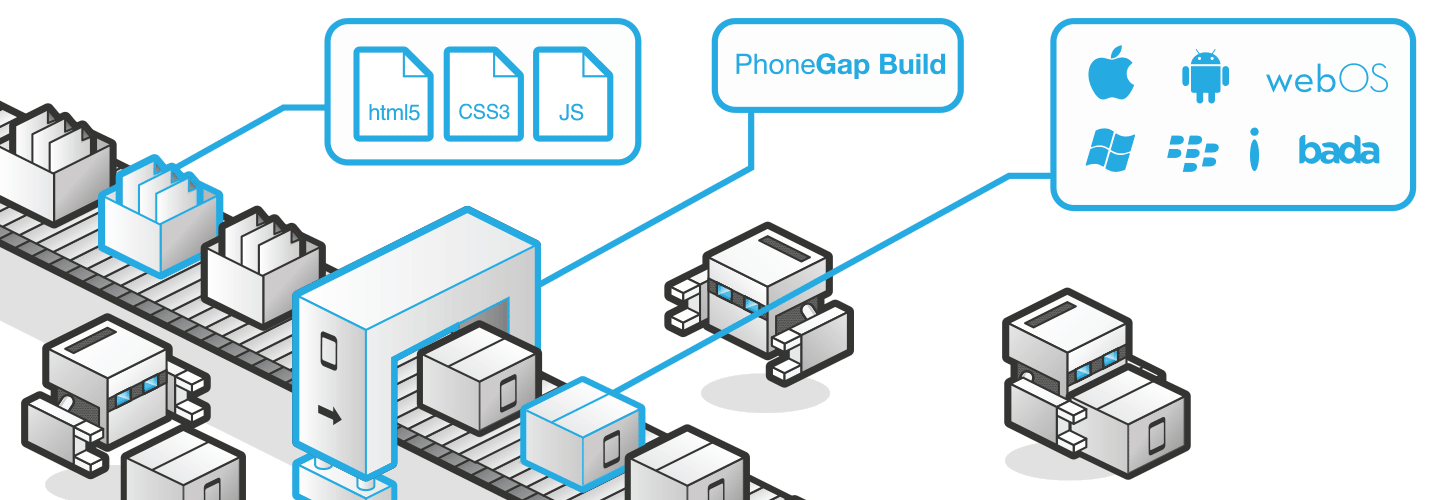
\includegraphics[scale=0.3]{Implementazione/phonegap_build.png}
	\caption{Logo del framework PhoneGap}
	\label{fig:phonegap_build}
\end{figure}

\newpage
Ora illustriamo mediante la Figura \ref{fig:architettura_phonegap} come è strutturata l'architettura PhoneGap. Partendo dal basso verso l'alto, si può notare che la parte in blu è quella del sistema operativo della piattaforma nativa che si trova sui vari device. Al livello immediatamente successivo troviamo il framework PhoneGap (in grigio) che ci viene fornito insieme alle API Javascript. Da notare il rettangolo arancione che rappresenta l'embedded browser che incapsula la web application e le API. Di default il browser viene aperto esternamente all'applicazione. Di conseguenza ad ogni richiesta di una pagina web avviene l'apertura di un bottone fornito dal browser. In pratica si rende impossibile notare che si tratta di un browser e quindi di una pagina web. Ciò rende l'applicazione più simile ad un applicazione nativa.\\
Infine, in verde è evidenziata la parte a carico dello sviluppatore che è la vera e propria web application, realizzata all'interno del framework PhoneGap.
\begin{figure}[H]
	\centering
	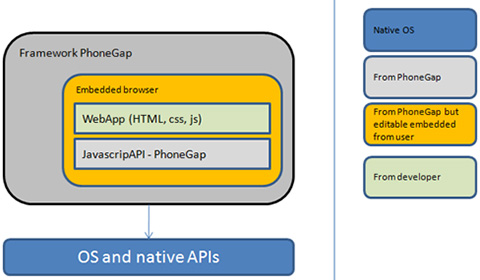
\includegraphics[scale=0.9]{Implementazione/phonegap_architettura.jpg}
	\caption{Architettura di un'applicazione realizzata con PhoneGap}
	\label{fig:architettura_phonegap}
\end{figure}

Come detto PhoneGap mette a disposizione del programmatore, una serie di API per l'accesso all'hardware nativo del device. Bisogna tenere conto però che non tutte le piattaforme hanno a disposizione gli stessi sensori e che occorre prestare molta attenzione nel caso in cui il building dell'applicazione è fatto su piattaforme diverse. Il framework, infatti, offre supporto per ogni piattaforma degna di essere presa in considerazione ovvero: Android, iOS, Symbian, WebOS, Blackberry etc. Non tutte le piattaforme son però supportate allo stesso modo. La seguente tabella (Fig \ref{fig:tabella_api} )
riassume lo stato dell'arte riguardo la compatibilità e l'accessibilità che il framework offre verso i sensori presenti nei diversi device, equipaggiati da diversi OS.

\begin{figure}[H]
	\centering
	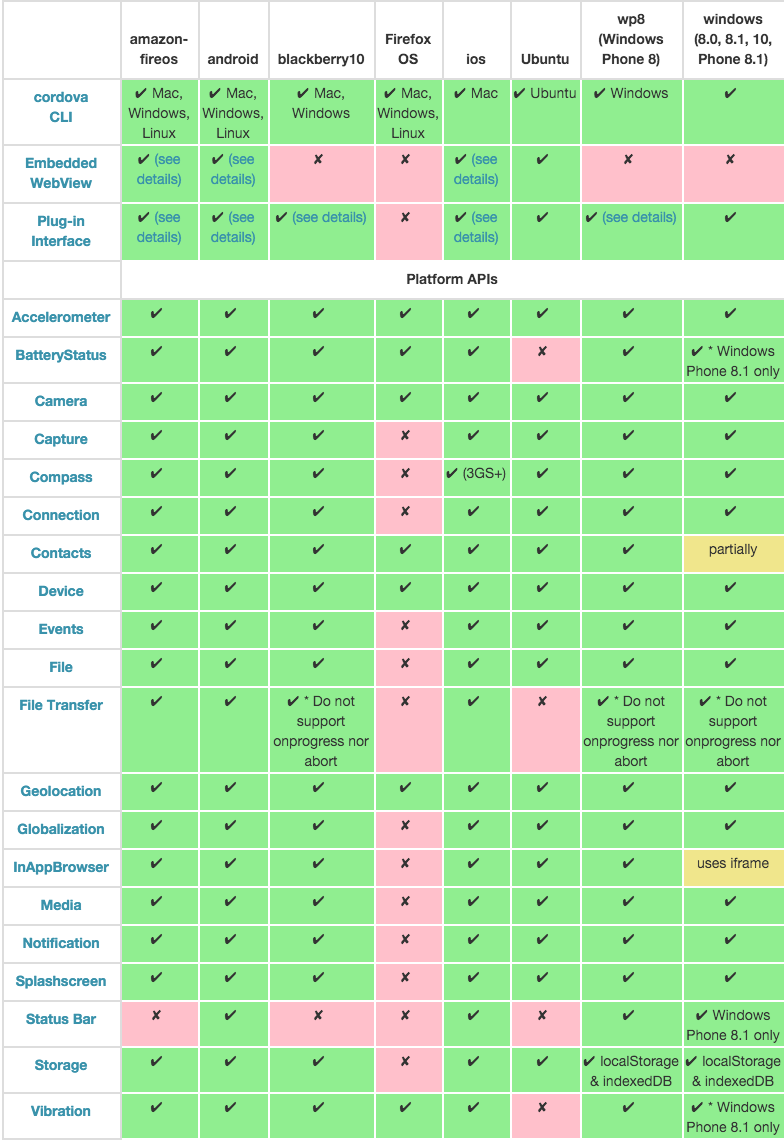
\includegraphics[scale=0.8]{Implementazione/phonegap_api.png}
	\caption{Le API e il loro supporto per le varie piattaforme}
	\label{fig:tabella_api}
\end{figure}

\section{Ratchet}
Il solo utilizzo del framework PhoneGap non è sufficiente per realizzare un'applicazione degna di nota. L'interfaccia grafica costituisce un'elemento fondamentale nelle moderne applicazioni mobili. Inoltre, se ben progettata, contribuisce ad aumentare la user experience \cite{EXPERIENCE} e in generale l'usabilità del sistema stesso. A tale proposito è stato utilizzato il framework opens source \textbf{Ratchet} [http://goratchet.com/].

\begin{figure}[H]
	\centering
	
\includegraphics[scale=1]{Implementazione/ratchet_logo.png}
	\caption{Il logo del framework Ratchet}
	\label{fig:logo_ratchet}
\end{figure}

I componenti grafici offerti da questo strumento sono responsive e appositamente progettati per gli smartphone; il loro utilizzo è tanto semplice quanto efficace, analogamente ad altri progetti di successo, come Bootstrap, i componenti possono essere inclusi nell'interfaccia aggiungendo dello specifico codice HTML e vari stili CSS (costumizzabili a proprio piacimento). A partire dalla seconda versione è stata integrata una classe di icone con immagini di uso comune nelle applicazioni mobili.\\
La combinazione di questo tool insieme ad altri per l'accesso al DOM (Document Object Model) dell'applicazione (vedi \ref{phonegap}), nel nostro caso \textit{jQuery}, permette di realizzare applicazioni con un'interfaccia accattivante e molto simile a quelle native.
\newpage
Ad esempio per aggiungere la "classica" tab-bar basta inserire il seguente codice HTML:
\begin{lstlisting} [language=XML]
<nav class="bar bar-tab">
  <a class="tab-item active" href="#">
    <span class="icon icon-home"></span>
    <span class="tab-label">Home</span>
  </a>
  <a class="tab-item" href="#">
    <span class="icon icon-person"></span>
    <span class="tab-label">Profile</span>
  </a>
  <a class="tab-item" href="#">
    <span class="icon icon-star-filled"></span>
    <span class="tab-label">Favorites</span>
  </a>
  <a class="tab-item" href="#">
    <span class="icon icon-search"></span>
    <span class="tab-label">Search</span>
  </a>
  <a class="tab-item" href="#">
    <span class="icon icon-gear"></span>
    <span class="tab-label">Settings</span>
  </a>
</nav>
\end{lstlisting}
\newpage
Ed ottenere il seguente risultato:
\begin{figure}[H]
	\centering
	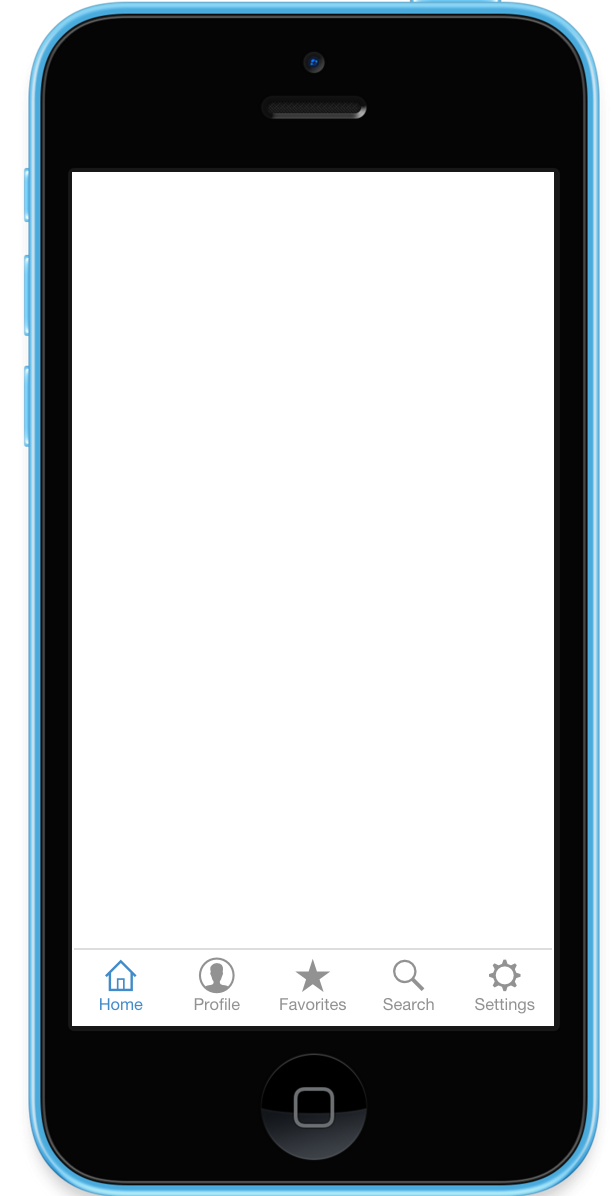
\includegraphics[scale=0.7]{Implementazione/tab-bar.png}
	\caption{Il componente tab-bar con cinque icone}
	\label{fig:tab}
\end{figure}

\newpage

\section{La griglia trasparente}
Come specificato nei requisiti di sistema, l'utente e gli eventi devono essere associati in modo univoco ad una cella di larghezza (22 x 16) mt; per fare ciò è necessario che il sistema sia in grado di "costruire" una griglia. Questa deve essere del tutto invisibile agli utenti che non hanno alcun interesse a conoscere o comprendere tale dettaglio.\\
Prima di spiegare la soluzione a questo problema occorre fare un passo indietro, sin dai tempi più remoti l'uomo ha cercato di creare delle mappe cartografiche. Le più antiche testimonianze \cite{GROTTE} conosciute di qualcosa che assomigli ad una rappresentazione cartografica non riguardano la terra, ma il cielo, così come appare di notte. Sui muri delle grotte di Lascaux sono stati infatti osservati dei puntini dipinti databili al 16.500 a.C.che rappresentano il cielo notturno ed in cui si possono riconoscere Vega, Deneb e Altair (il cosiddetto Triangolo estivo), nonché le Pleiadi.Dall'ora la cartografia ha fatto passi da gigante(vedi \ref{OpenStreetMap}).\\
Tornando a noi, la soluzione trovata si basa sul calcolo della distranza tra due punti geografici, il cui problema è la definizione stessa dei punti. Non avendo la Terra una forma lineare, è difficile trovare una rappresentazione geometrica perfetta di essa. \\
Gli algoritmi più utilizzati per il calcolo della distanza tra due punti, utilizzano le formule di Haversine e Vincenty, il primo si basa sull'approssimazione della terra ad una sfera perfetta, mentre il secondo la modelizza in uno sferoide oblato. \\
E' bene dire che mentre il risultato ottenuto tramite la formula di Haversine può avere un'errore dello 0,3\%  quello di Vincenty è molto più accurato, con un errore di 0.5mm circa; questa precisione si ha a discapito di un costo computazionale più elevato. Per brevi distanze i metodi tendono invece a convergere.\\
Con entrambi gli algoritmi è stato verificato che una variazione unitaria di $10^{-4} $ gradi corrisponde ad una distanza di 11 mt se in latitudine, 8 mt se in longitudine. Partendo da questo risultato si è così ideato \textbf{l'algoritmo di Santiago}.
\newpage
\begin{enumerate}
\item L'utente viene "posto" all'interno di un sistema di riferimento calcolato troncando la sue coordinate alla $10^{-3} $ cifra decimale. La grandezza fisica dei sistemi è $ 110* 88 mt^{2} $. L'origine corrisponde alle coordinate dell'utente troncate alla $10^{-4} $, con l'ultima cifra decimale uguale a zero.
\begin{figure}[H]
	\centering
	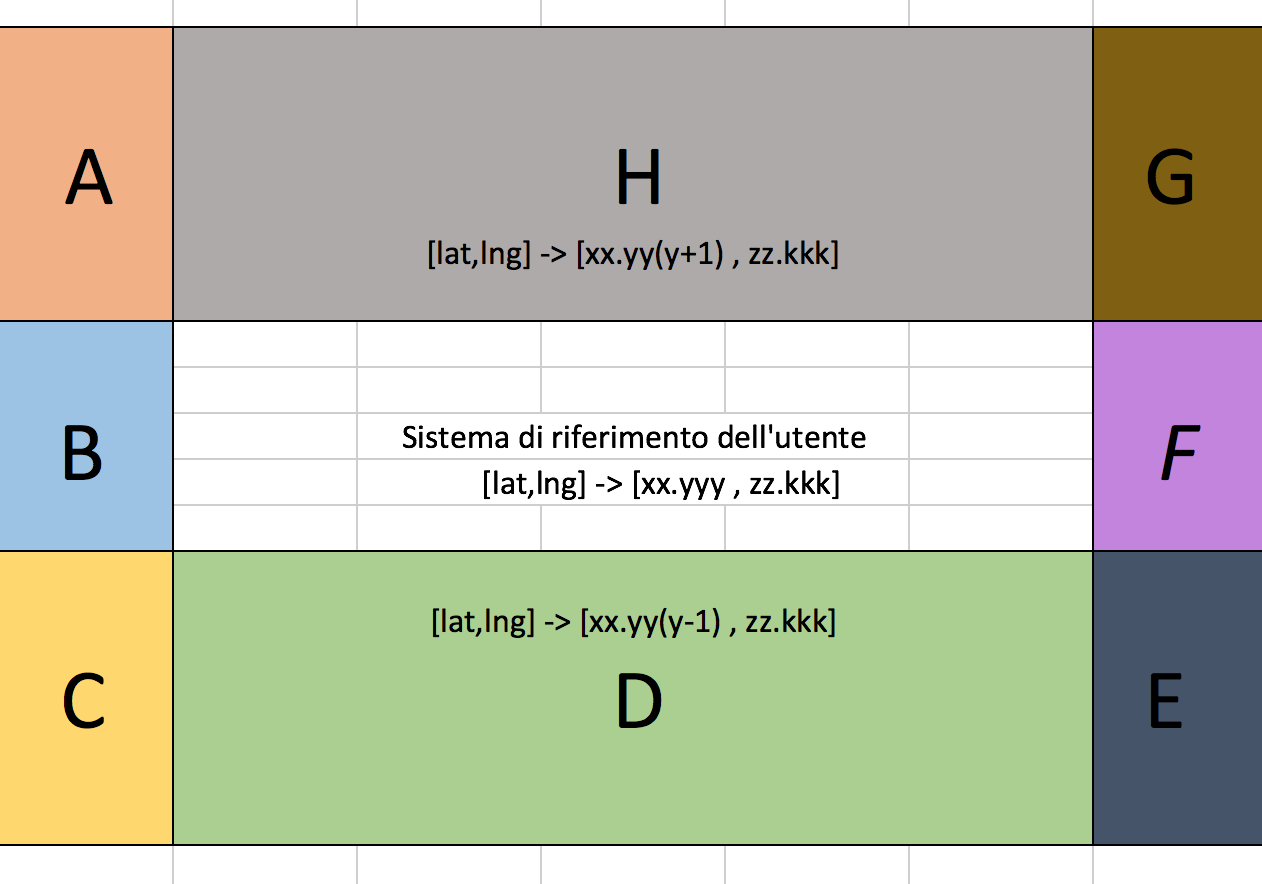
\includegraphics[scale=0.6]{Implementazione/sis1.png}
	\caption{Sistema di riferimento dell'utente}
	\label{fig:sis}
\end{figure}
\newpage
\item Le coordinate dell'utente (o dell'evento) vengono troncate definitivamente alla quarta cifra decimale, questo significa mappare tutte le persone all'interno di rettangolo di grandezza $11 * 8 mt^{2}$ nell'angolo in basso a destra (ndr Santiago de Chile si trova in direzione sud-ovest dall'Italia, da cui il nome dell'algoritmo) con le prime tre cifre decimali uguali e l'ultima uguale a zero. Di seguito un'immagine per chiarire meglio il funzionamento.

\begin{figure}[H]
	\centering
	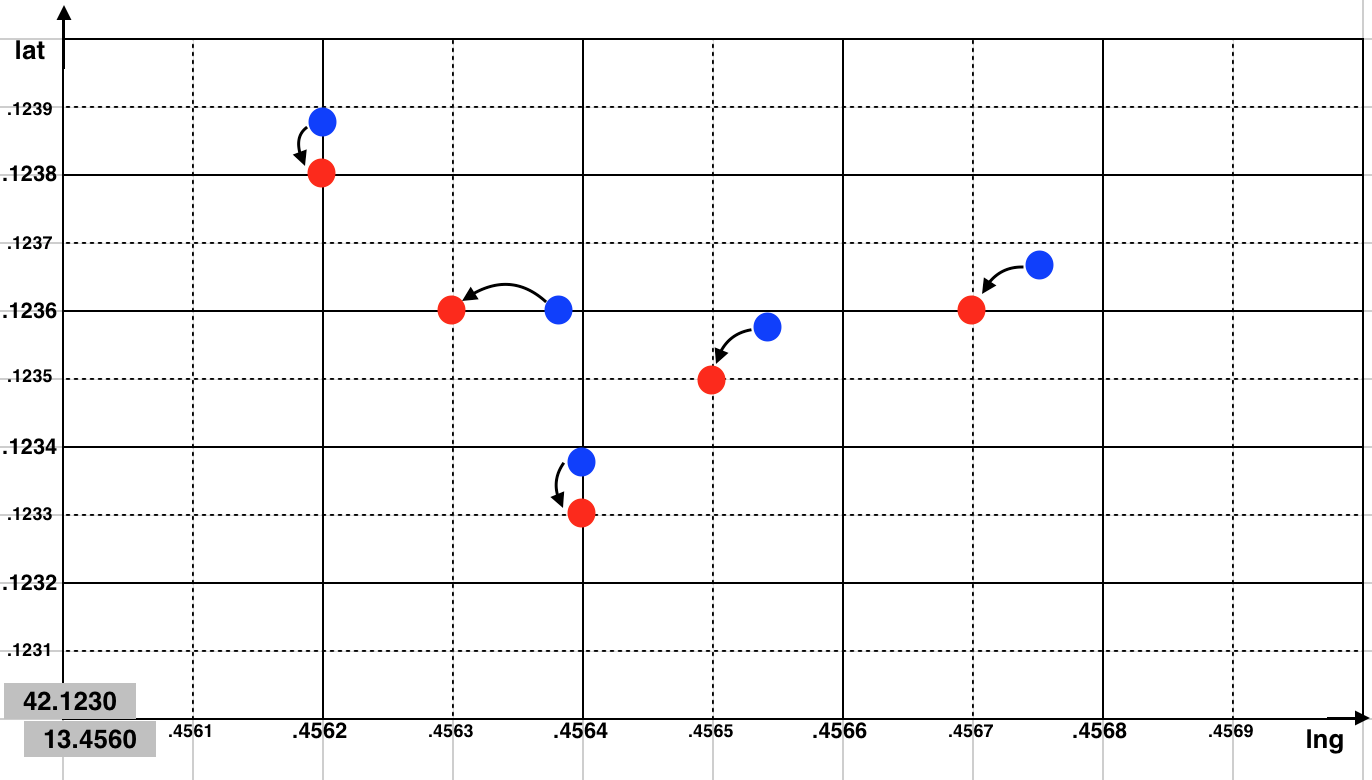
\includegraphics[scale=0.6]{Implementazione/mapping.png}
	\caption{Mapping dell'utente all'interno delle celle}
	\label{fig:mapping}
\end{figure}
\end{enumerate}

I cerchi blu rappresentano le posizioni di diversi utenti, mentre i cerchi rossi rappresentato la posizione dopo il troncamento.
\newpage

\item Per rispettare le specifiche le celle devono essere composte da quattro celle (in fig \ref{fig:mapping} racchiuse da bordi neri continui)



\chapter{Conclusioni e prospettive future}

Come già detto, l'obiettivo di questa tesi è lo sviluppo di un'applicazione mobile cross-platform geolocalizzata per contesti di disaster-management. Pur avendo realizzato l'interfaccia e le principali funzioni del sistema, il lavoro non può considerarsi terminato. \\
In particolare non si è avuto il tempo di affrontare le seguenti questioni:
\begin{itemize}
\item \textbf{GPS device}: al fine di realizzare un'applicazione affidabile, come il contesto applicativo richiede, bisogna condurre uno studio dettagliato sulla precisione e il funzionamento della tecnologia GPS dei dispositivi mobili.
\item \textbf{Usabilità}: gli utenti appartengono ad un'ampia fascia di età, per questo motivo occorre effettuare un test di usabilità del sistema e nell'eventualità modificare/riprogettare l'interfaccia.
\item \textbf{Buffering}: come stabilito nei requisiti, in caso di rete congestionata o assente il sistema deve bufferizzare le richieste e informare l'utente. Bisogna progettare un algoritmo efficente e un'opportuna struttura dati, in modo tale da sfruttare al meglio le risorse limitate dei dispositivi mobili.
\item \textbf{Ping dispositivo}: un'ulteriore informazione sugli utenti è data dallo stato del dispositivo, variabile tra: power-off, power-on e online. Per fare ciò, il server deve periodicamente "pingare" gli utenti. In futuro il progettista del server dovrà necessariamente implementare questa funzione.
\item \textbf{Update dati}: a causa della mancanza di un server, i dati presenti nell'applicazione sono statici. Sappiamo invece che nel contesto applicativo i dati sono dinamici (vedi \ref{contesto}). L'applicazione dovrebbe richiedere l'aggiornamento dei dati in modo intelligente, ovvero bisogna progettare un algoritmo che, considerando il numero di utenti all'interno del sistema e lo stato della rete, determi la periodicità delle richieste per ogni utente.
\end{itemize}
Una volta realizzato interamente il sistema ideato dal team di ricerca (vedi \ref{contesto}), questa applicazione svolgerà un ruolo cruciale nella ricerca e assistenza delle vittime di un disastro ambientale e/o umano, contribuendo in generale ad aumentare la resilienza della comunità nei luoghi in cui tale progetto sarà implementato.



\chapter*{Ringraziamenti}
\markboth{Ringraziamenti}{Ringraziamenti}
\addcontentsline{toc}{chapter}{Ringraziamenti}
\thispagestyle{empty}

Desidero ringranziare sentitamente il prof. Giovanni De Gasperis per i preziosi consigli e il tempo dedicatomi. Inoltre desidero ringraziare la prof.ssa Laura Tarantino per avermi proposto questo affascinante lavoro e per i suoi utili insegnamenti, i quali hanno contribuito significativamente alla mia attuale formazione professionale come ingegnere.\\
Inoltre desidero ringraziare i miei amici e la mia compagna per avermi supportato durante tutto il mio percorso. Infine dedico questo e tutti i miei futuri successi alla mia famiglia, il mio carburante, la mia unica variabile globale.


% BEGIN Bibliografia
\begin{thebibliography}{99}
\addcontentsline{toc}{chapter}{Bibliografia}

\bibitem{NOTE}
Theoretical Notes on Vulnerability to Disaster
\url{http://emergency-planning.blogspot.it/2009/01/theoretical-notes-on-vulnerability-to.html}

\bibitem{COMMON}
Fifty-six Common Misconceptions About Disaster
\url{http://emergency-planning.blogspot.it/2008/12/forty-four-common-misconceptions-about.html}

\bibitem{FASI_MANAGEMENT}
Phases of Emergency Management
\url{http://www.cheltenhamtownship.org/mobile/pview.aspx?id=4161&catid=29}

\bibitem{RESPONSE}
Disaster Response: a Multi-Agent based Approach,
\url{http://www.sapienzaapps.it/chitaly2015/wp-content/uploads/2015/09/02_chitaly2015_Costantini_et_al.pdf}


\bibitem{LICENZA_OSM}
Open Data Commons  \\
\url{http://opendatacommons.org/licenses/odbl/summary/}

\bibitem{MAPPE_LIBERE}
wiki.openstreetmap, ``Perché state realizzando OSM?'' \\
\url{http://wiki.openstreetmap.org/wiki/IT:FAQ}

\bibitem{WHYNEED}
Why the world needs OpenStreetMap, ``Perché il mondo ha bisogno di OSM?''
\url{http://www.theguardian.com/technology/2014/jan/14/why-the-world-needs-openstreetmap}

\bibitem{ACCURATEZZA_MAPPE}
wiki.openstreetmap, ``Com'è possibile che un progetto del genere porti a mappe accurate?'' \\
\url{http://wiki.openstreetmap.org/wiki/IT:FAQ}

\bibitem{GOOGLE_PLAN}
Google Developers ,  ``JavaScript API Usage Limits''
\url{https://developers.google.com/maps/pricing-and-plans/}


\bibitem{GOOGLE_OFFLINE}
Google Support ,  ``Download e utilizzo di aree offline''
\url{https://support.google.com/gmm/answer/6291838?hl=it}

\bibitem{LINK_PLANET}
Wiki OSM,  ``Planet.OSM"
\url{https://wiki.openstreetmap.org/wiki/Planet.osm}

\bibitem{HOT_PROJECT}
Humanitarian Openstreetmap Team,  ``Disaster Mapping"
\url{https://hotosm.org/projects/disaster-mapping}

\bibitem{WIKI_HAITI}
Terremoto di Haiti del 2010
\url{https://it.wikipedia.org/wiki/Terremoto_di_Haiti_del_2010}

\bibitem{EXPERIENCE}
User Experience
\url{https://it.wikipedia.org/wiki/User_Experience}




\end{thebibliography}




% END Bibliografia


\end{document}